\chapter{Physics Formalism}
\label{ch:physrev}
The idea that matter is made of elementary particles has been around since about the 6th Century B.C.E., but it was not until 2400 years later in 1808 \cite{book:dalton} that the first publication came out by John Dalton describing small particles called atoms. Between 1879 \cite{crookes} and 1897 \cite{thomson} works that discovered the existence of electrons started to be published and taken seriously. By 1914, Rutherford \cite{book:rutherford1} and others established that there was a dense structure at the center of atoms that had a positive charge surrounded by the lighter-mass electrons on the outside. In 1913, the positively charge $nucleus$ of the hydrogen atom was confirmed by Rutherford \cite{book:rutherford2}, which he named $proton$. It was not until 1932 that James Chadwick discovered the neutron.

Alongside the discoveries of these subatomic particles was the development of theories explaining their behavior. Electrons began to be understood as both a particle and a wave, depending on which way you try to observe it. Then it was realized all particles can act this way. Max Plank developed the idea that energy radiated from atomic systems did so only in discrete quantities or $quanta$. In 1905, Einstein \cite{einstein} proclaimed that light is made of particles called photons, which was consistent with Plank's $quantum$ hypothesis. Throughout the early 1900's this concept of quantum mechanics was developed.

In this journey through understanding the quantum world came the realization that the four fundamental forces in nature ($i.e.$ gravity, electromagnetic, strong and weak nuclear) are fields that interact with quantum particles, which were also considered fields. For the electromagnetic force, this became known as quantum electrodynamics (QED) developed around the 1950-1960's. The interactions of particles with the strong nuclear force were described by a theory called quantum chromodynamics (QCD) developed around the late 1970's. This chapter will, in effect, follow this history with a slant toward its relevance in the BONuS12 Experiment.

\section{Nucleon Structure}
The proton and neutron are the two components that make up a group called nucleons since they make up the nucleus of an atom. They both interact through all four forces ($i.e.$ strong nuclear, weak nuclear, electromagnetic, and gravitational). As mentioned in the Introduction, they are both fermions. Because they are both made up of three quarks, they are also both baryons.

The quarks that make up these nucleons (all baryons, in fact) and that are responsible for the nucleon's quantum numbers are called \textit{valence quarks}. The proton is made of two \textit{up} valence quarks and one \textit{down} valence quark, denoted by $uud$. The neutron is made up of two down valence quarks and an up valence quark, or $udd$. Of course, there are also \textit{sea quarks} made of $q\bar{q}$ pairs, where $q\bar{q}$ is any variety of quark-antiquark pair. However, the strong interaction which binds all of these quarks together acts the same no matter the quark flavor.\footnote{The word \textit{flavor} is used to describe a type of quark. Remember there are 6 \textit{flavors} of quarks: up, down, top, bottom, strange, and charm.} Therefore, the quark model does not predict any distinctions between protons and neutrons. In fact, from the view of the strong force, they are the identical particle in different states.\footnote{There is a symmetry of the strong interaction in neutrons and protons called isospin (also referred to as isotopic or isobaric spin). Isospin is a dimensionless quantity that does not describe a physical ``spin" of the particle. It does, however, offer a description of the two different states of nucleons. In particular, the projection of isospin along the z-axis ($I_z$ or $I_3$) provides insight into the difference between protons and neutrons, which are otherwise almost identical particles. Protons have $I_z=1/2$ and neutrons have $I_z=-1/2$.} Yet, protons and neutrons are clearly not identical particles.

There are obvious differences between the two nucleons. One important difference between nucleons is their stability when not bound to each other. The proton is a stable particle on its own, with a lifetime of more than $2.1 \times 10^{29}$ years. The neutron, however, has a lifetime of about $882$ seconds (or about 15 minutes). The proton is the only nucleon that can exist in a nucleus on its own, such as in the hydrogen atom. The obvious difference in the two nucleons is their electric charge. The charge of the proton is $+1$ in units of electron charge, while the neutron is neutral ($i.e.$ charge = 0). This charge arises from their valence quark content. The up quark has a charge equal to $q_u = +2/3$ and the down quark has a charge of $q_d = -1/3$, so for the proton with $uud$ quarks,

\begin{equation}
2q_u + q_d = 2(+2/3) + (-1/3) = +1,
\end{equation}
and for the neutron with $ddu$ quarks,

\begin{equation}
2q_d + q_u = 2(-1/3) + (+2/3) = 0.
\end{equation}
The spatial charge distribution of quarks is well known for both nucleons. The momentum distribution of those quarks inside the nucleon is not as well known, especially for the neutron. The same is true for the overall structure of the nucleons, again more so for the neutron.

\begin{figure}[h!]
	\centering
	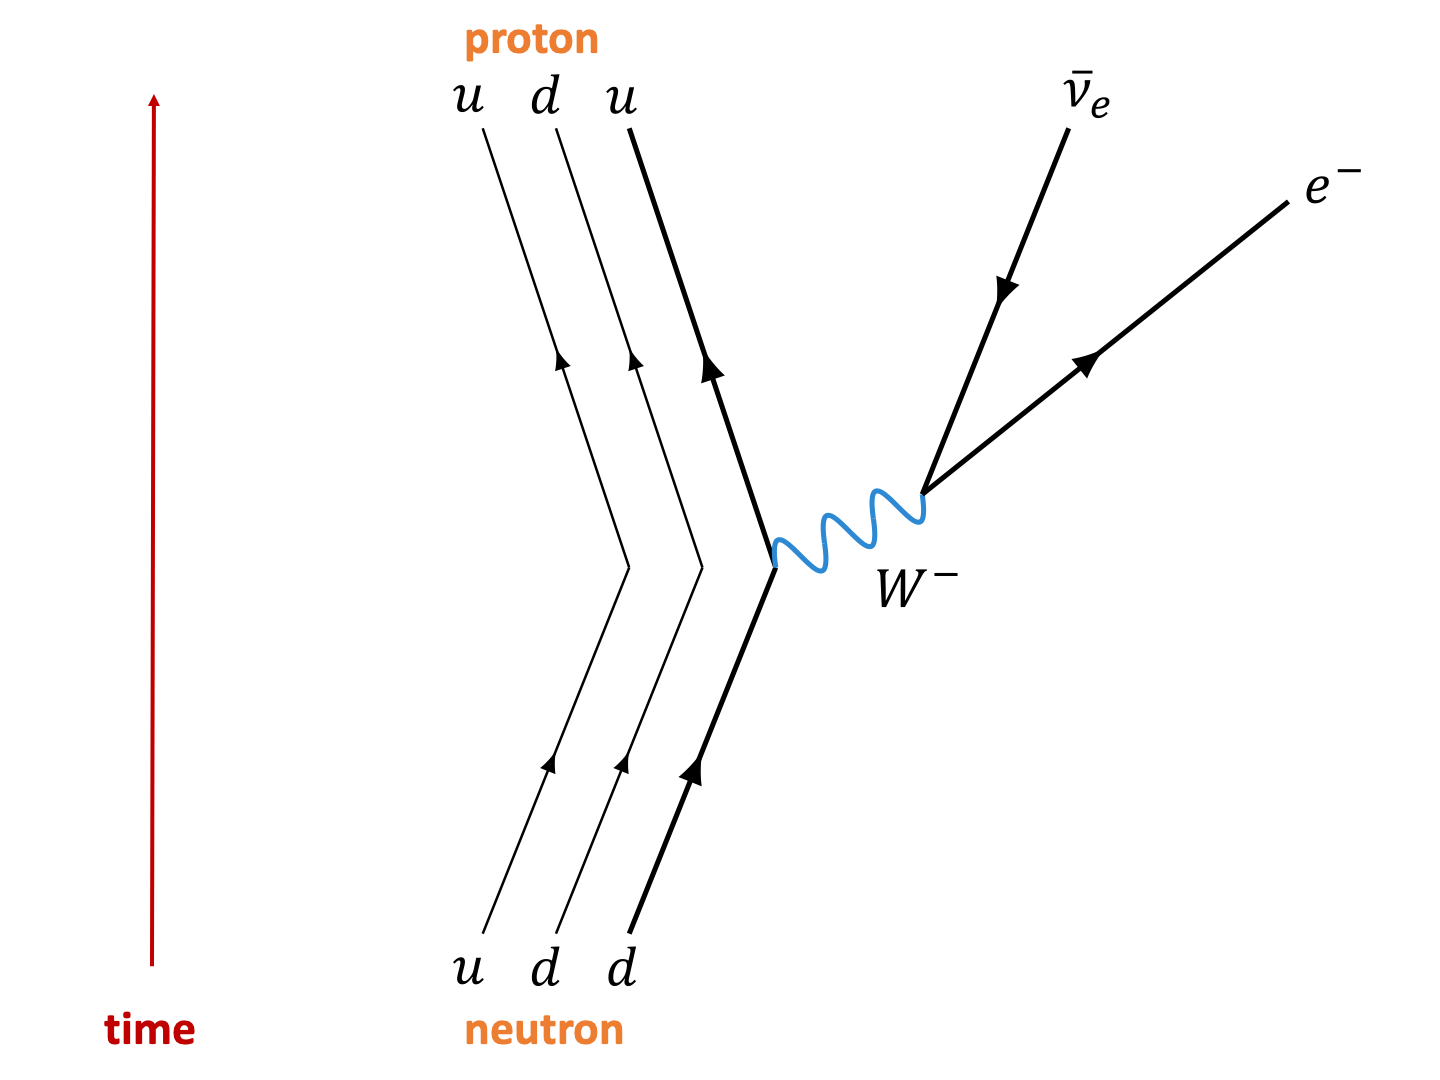
\includegraphics[width=0.6\linewidth]{figures/neutron_decay.png}
	\caption{The Feynman diagram of neutron decay.}
	\label{fig:neutron_decay}
\end{figure}

The discrepancy of knowledge between the proton and the neutron is the last major difference of the nucleons we will discuss here, because it goes directly toward the principle goal of the BONuS12 Experiment. We know much more about the structure of the proton and momentum distribution of the quarks inside the proton for the reason discussed in the last paragraph. That is, protons can exist outside of nuclei while neutrons soon decay via the weak interaction

\begin{equation}
n \longrightarrow p + e^{-} + \bar{\nu}_{e},
\end{equation}
as seen in Fig. \ref{fig:neutron_decay} as a Feynman diagram. Feynman diagrams were developed by physicist Richard Feynman to display particle interactions that occur in a relatively simplistic manner. Moving from the bottom to the top in the diagram of Fig. \ref{fig:neutron_decay}, we see a down quark within the neutron change states to an up quark mediated by the $W^-$ boson, which then decays to an electron ($e^-$) and electron antineutrino ($\bar{\nu}_{e}$). This neutron decay occurs in 15 minutes. That decay coupled with the fact that the neutron has no electric charge makes isolating neutrons to create a target for scattering experiments extremely difficult. Yet, scattering experiments are the primary means by which physicists study the structure of particles. Therefore, studying the structure of the neutron is inherently made difficult by this lack of free neutron target.

\section{Electron-Scattering Kinematics}
To study the structure and physics of particles, nuclear and particle physicists use scattering experiments. There are two ways of creating a scattering experiment. One way is to accelerate a light particle (an electron, for example) and direct it toward a stationary target, which is the method used at Jefferson Lab in Newport News, Virginia. The other way is to accelerate two particles in opposite directions and then direct the two toward each other, which is the method used at the Large Hadron Collider (LHC) at CERN in Geneva, Switzerland. The physics or kinematics\footnote{The word kinematics refers to the mechanics of the particles without concern for the forces that caused the motion. Essentially, we are not concerned with \textit{how} the particles were accelerated, just that they have a particular energy at the time of collision.} of both scattering experiments is essentially the same. 

When the scattering particle and target collide, some of the momentum and energy of the scattering particle is transfered to that target particle. Nuclear and particle physicists express that energy and momentum as a four-momentum. Classical momentum is a vector, which means it has a magnitude and direction. That direction is typically expressed in three dimensions (for the familiar Cartesian coordinate system that would be along the x, y, and z-axis). Therefore a momentum can be expressed as $\mathbf{p}$ = ($p_x$, $p_y$, $p_z$), where $\mathbf{p}$ is the momentum vector bold-faced to indicate that it is a vector. Because in particle physics, the particles travel close to the speed of light, we have to deal with special relativity. For the purposes of this work, special relativity essentially forces us to consider not just three-dimensional space, but four dimensional space-time with different reference frames for any non-accelerating moving objects. This drives us to require there be a four-dimensional space-time momentum $p=(p_0,p_1,p_2,p_3)$, where $p_1=p_x$, $p_2=p_y$, and $p_3=p_z$ in Cartesian coordinates. The new term $p_0$ is equal to $E/c$, where $E$ is the energy of the particle and $c$ is the speed of light.

If we take this four-momentum
\begin{equation}
p_{\mu} = \left( \frac{E}{c}, p_x, p_y, p_z \right),
\end{equation} 
where $\mu$ is just an index indicating a particular particle, and square it, we have
\begin{equation}
p^{\mu}p_{\mu} = -\frac{E^2}{c^2} + p^2_x +p^2_y + p^2_z = -\frac{E^2}{c^2} + \mathbf{p}^2.
\end{equation}
This quantity is invariant under a Lorentz transformation (meaning it remains the same no matter the non-accelerating reference frame) and is equal to the Lorentz scalar $-m^2c^2$, which means 
\begin{equation}
\label{eqn:4mom}
-\frac{E^2}{c^2} + p^2 = -m^2c^2.
\end{equation}
Multiplying both sides of Eq. \ref{eqn:4mom} by $-c^2$ and rearranging a little gives us
\begin{equation}
\label{eqn:e_squared}
E^2 = p^2c^2 + m^2c^4,
\end{equation}
which if we take the square root of both sides results in
\begin{equation}
E=\sqrt{(pc)^2+(mc^2)^2}.
\end{equation}
In the rest frame of the particle ($i.e.$ the frame where the particle is considered to have no momentum, thus $p=0$), this equation reduces to something that should be familiar:
\begin{equation}
E=mc^2.
\end{equation}
This rough derivation provides a little insight to the power and purpose of using four-momentum. We will use this notation extensively throughout the rest of this work. 

The other useful notation to understand is called natural units, where $c=\hbar=1$. Under these units, Eq. \ref{eqn:e_squared} becomes
\begin{equation}
E^2 = p^2 + m^2.
\end{equation}
While this offers much in the way of simplicity when working with complex equations, the disadvantage is that we lose information regarding dimensional analysis of the equation. Nevertheless, for the most part, we will use natural units in this work.

Consider an electron with four-momentum $k$ scattering off of a nucleon with momentum $p$. The Feynman diagram for such an interaction is in Fig. \ref{fig:feyn_epscatt}, where $k'$ and $p'$ are the final momentum of the scattered electron and nucleon respectively. Here, $q$ is the momentum of the virtual photon\footnote{The term ``virtual" here may be misleading. It does not imply that the photon does not really exist. It refers to the short-lived exchange of the electromagnetic force.} (typically denoted by $\gamma^{*}$) that mediates the interaction. That virtual photon momentum, $q=k'-k$, is the momentum lost by the scattered electron.

\begin{figure}[h!]
	\centering
	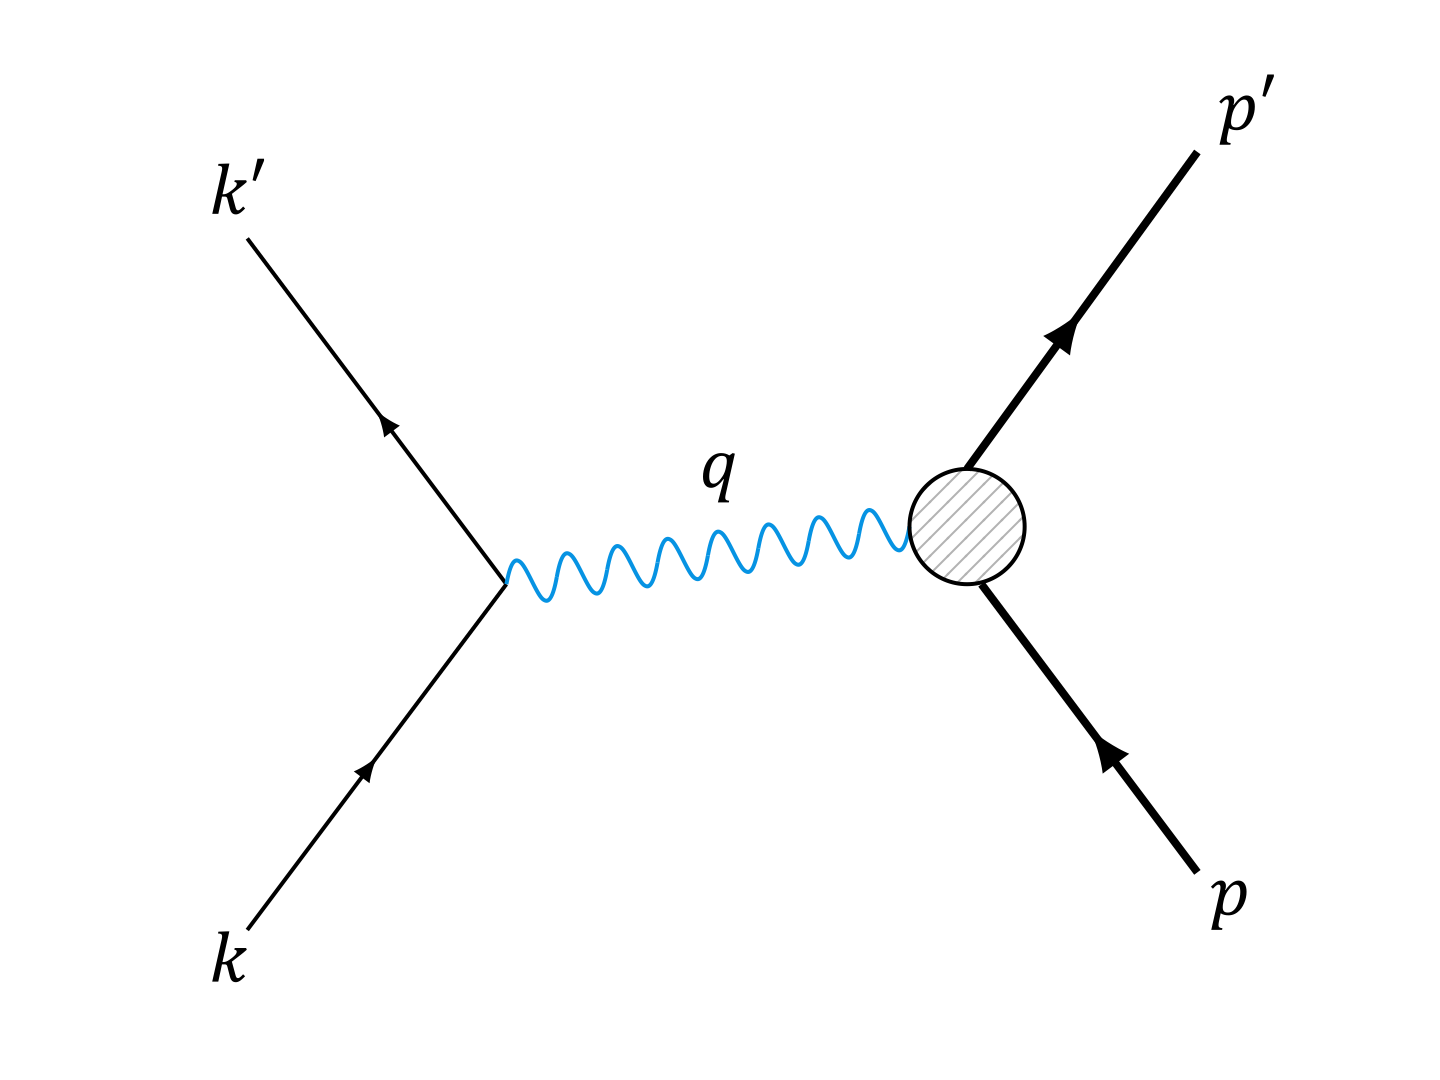
\includegraphics[width=0.6\linewidth]{figures/feyn_epscatt.png}
	\caption{Feynman diagram of an electron scattering from a proton.}
	\label{fig:feyn_epscatt}
\end{figure}

There are some other important quantities to consider for electron scattering. The first is the square of that four-momentum transfer
\begin{equation}
q^2 = (k' - k)^2 = 2m_e^2 - 2(EE' - |\mathbf{p}||\mathbf{p}'| \cos \theta),
\end{equation}
where $m_e$ is the mass of the electron, $E$ is the energy of the incident electron, $E'$ is the energy of the scattered electron, $|\mathbf{p}|$ is the magnitude of the three-momentum of the incident nucleon, $|\mathbf{p}'|$ is the magnitude of the scattered nucleon's three-momentum, and $\theta$ is the scattering angle of the electron. When we use the trigonometric identity $1-\cos \theta = 2 \sin^2 \tfrac{\theta}{2}$ and take the electron mass to be zero ($i.e.$ $|p| = E$), we get
\begin{equation}
q^2 \approx -4EE'\sin^2\tfrac{\theta}{2}.
\end{equation}
As a convention to make the quantity positive, we use $Q^2 = -q^2$, which will be used throughout the rest of this work. Another variable we need in order to analyze these electron scattering kinematics is the variable $\nu$, which is the energy transfer of the electron to the nucleon via $\gamma^*$ ($i.e.$ the virtual photon) and is defined by
\begin{equation}
\nu = \frac{p \cdot q}{M}.
\end{equation}
Here, $p$ is the four-momentum of the incident nucleon and $M$ is the nucleon mass. In the laboratory frame, the nucleon is at rest ($i.e.$ $p=(M,\mathbf{0})$)\footnote{Just like other three-dimensional vectors, when bolded, $\mathbf{0}$ represents (0,0,0).}, and $q=(E-E',\mathbf{q})$, so the energy transfered by the virtual photon to the nucleon in the laboratory frame would be
\begin{equation}
\nu  = E-E'.
\end{equation}

\begin{figure}[h!]
	\centering
	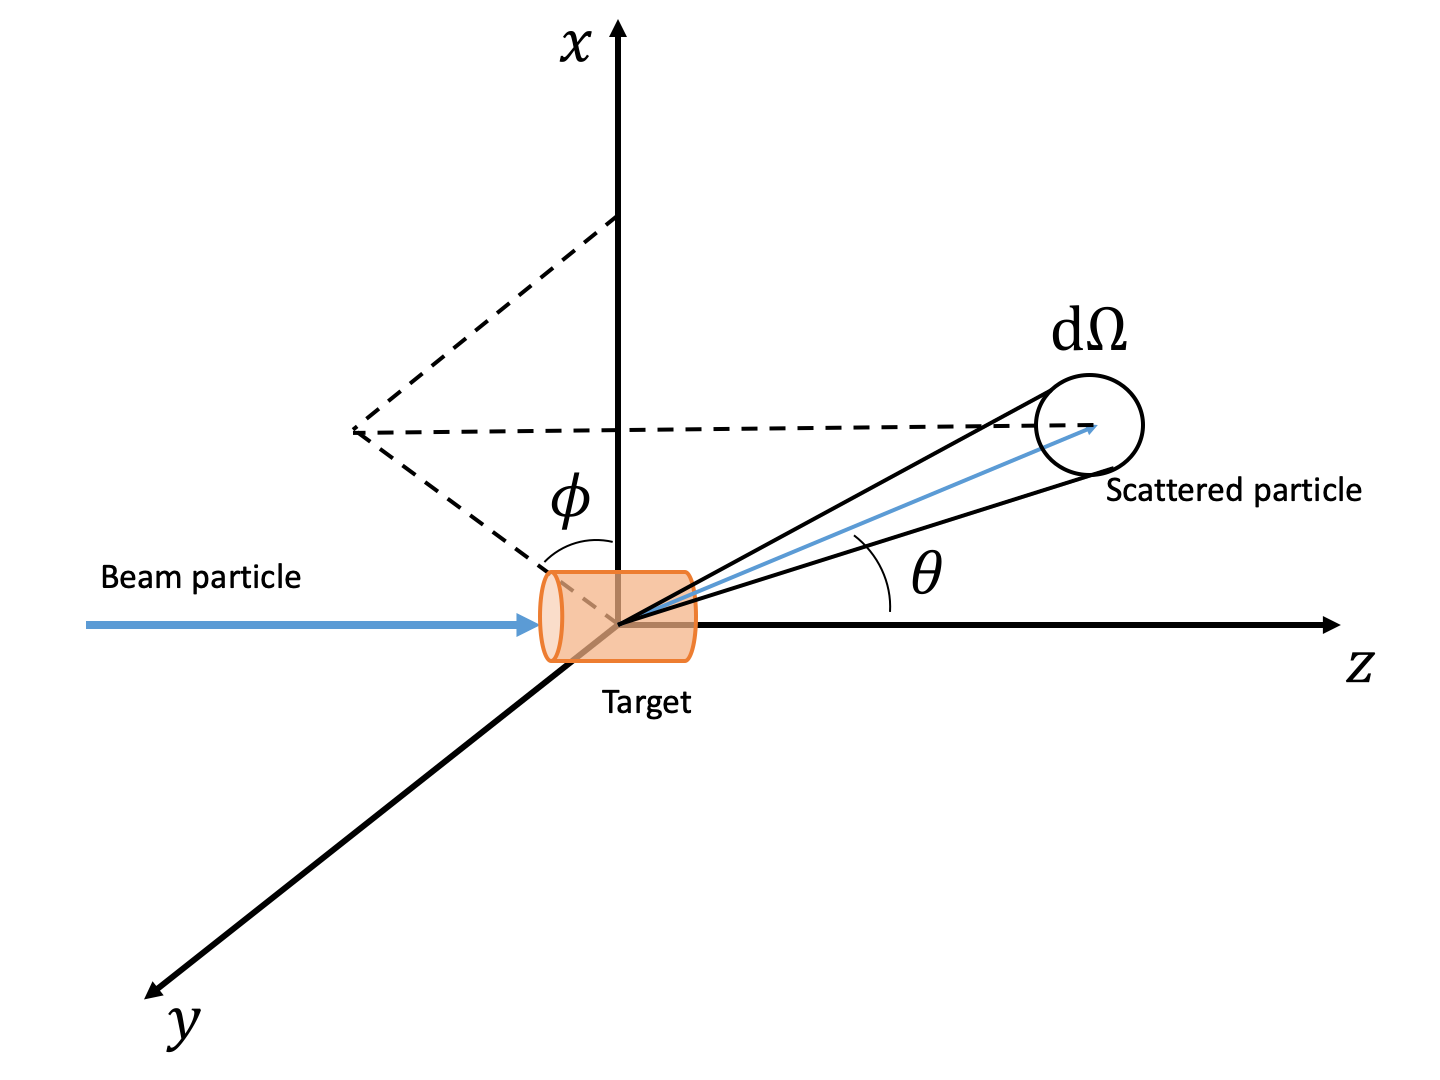
\includegraphics[width=0.6\linewidth]{figures/diff_xsec.png}
	\caption{Scattering process on a quasi-static differential cross section.}
	\label{fig:diff_xsec}
\end{figure}

Whenever we deal with collisions of particles, there is a probability associated with the reaction between that projectile and target depicted in Fig. \ref{fig:diff_xsec}. That probability is called the \textit{cross section} and with it often comes a wealth of knowledge about the dynamics of the interaction itself. In many reactions we deal with what is known as the \textit{differential} cross section, which reflects the fact that the probability of a reaction depends on the spatial or kinematic quantities. This differential cross section is the probability of particles scattered into a bit of the solid angle $\mathrm{d}\Omega$. Mathematically, the differential cross section for a spinless particle scattered from a static point charge can be written\cite{book:parts_nucs} as  
\begin{equation}
\label{eqn:rutherford}
\frac{\mathrm{d}\sigma}{\mathrm{d}\Omega} = \frac{\alpha^2}{4E^2\sin^4 \frac{\theta}{2}},
\end{equation}
where $\alpha$ is known as the fine-structure constant equal to $e^2/4\pi \approx 1/137$, $E$ is the energy of the incident electron, and $\theta$ is the scattering angle of the electron in the laboratory frame. Eq. \ref{eqn:rutherford} is known as the Rutherford Formula and is the simplest theoretical scattering case. If we include the electron spin, we get
\begin{equation}
\label{eqn:mott}
\frac{\mathrm{d}\sigma}{\mathrm{d}\Omega} = \frac{\alpha^2 \cos^2 \frac{\theta}{2}}{4E^2\sin^4 \frac{\theta}{2}},
\end{equation}
which is known at the \textit{Mott} cross section (we will from now on denote this particular cross section by $\left( \tfrac{\mathrm{d}\sigma}{\mathrm{d}\Omega} \right)_{\mathrm{Mott}}$). If we next introduce the mass of the point-like target $M$, that target particle will recoil, and so we get a scattered electron energy of 
\begin{equation}
E' = \frac{E}{1+\frac{2E}{M}\sin^2 \frac{\theta}{2}},
\end{equation}
and the Mott cross section becomes
\begin{eqnarray}
\nonumber
\frac{\mathrm{d}\sigma}{\mathrm{d}\Omega} =& \left( \frac{\mathrm{d}\sigma}{\mathrm{d}\Omega} \right)_{\mathrm{Mott}} \cdot \frac{E'}{E} \left[ 1-\frac{q^2}{2M^2}\tan^2 \frac{\theta}{2} \right] \\
=& \frac{\alpha^2 \cos^2 \frac{\theta}{2}}{4E^2\sin^4 \frac{\theta}{2}} \cdot \frac{E'}{E} \left[ 1-\frac{q^2}{2M^2}\tan^2 \frac{\theta}{2} \right].
\end{eqnarray}
As that target mass $M$ increases, this equation reduces to the Mott cross section. 

We are beginning to approach a more realistic mathematical description of scattering, so we must discuss the various types that exist. In Fig. \ref{fig:feyn_epscatt} if both particles remain intact in their ground state after the collision, it is called \textit{elastic scattering}. Like pool balls, they essentially bounce off each other, of course through the exchange of that virtual photon. Inelastic  scattering is when an internal excitation occurs in one or both particles. We need to understand these types of scattering in more depth to understand the BONuS12 Experiment.

\section{Elastic Scattering}
When the momentum transfer, or more specifically $Q^2$, is low, there is a higher probability that the lepton (at JLab, that lepton is an electron) essentially bounces off of the target particle (typically a nucleon) in what is known as elastic scattering. Whatever momentum is transferred does not force the nucleon into excited states (called resonances) or break it apart entirely (deep inelastic scattering). In a situation like Fig. \ref{fig:feyn_epscatt} when scattering elastically
\begin{equation}
k+p \longrightarrow k' + p'.
\end{equation}
Here $k$ and $p$ are the incident electron and nucleon four-momenta respectively, and $k'$ and $p'$ are the scattered electron and nucleon respectively. In this elastic case,
\begin{equation}
M_N = M'_N \; \; \mathrm{and} \; \; m_e = m'_e
\end{equation}
where $M_N$ is the mass of the nucleon and $m_e$ is the mass of the electron. 

Because the nucleon target not point-like, we cannot simply use the Mott Equation (Eq. \ref{eqn:mott}) to calculate the cross section of this elastic-scattering process. If we scatter electrons from some particle with a charge distribution $\rho(r)$ ($r$ distance away from the charge source), like a proton, the scattering amplitude (following \cite{book:halzen}) is modified by a form factor
\begin{equation}
\label{eqn:ff}
F(q^2) = \int d^3r \; e^{i\mathbf{q} \cdot \mathbf{r}} \; \rho(r).
\end{equation}
This particular form factor in Eq. \ref{eqn:ff} is an integral over volume of that charge distribution times the plane-wave representation of the particle. $F(q^2)$ is the Fourier transform of the charge distribution. As the name suggests this form factor provides insight into the composite structure of that particle. When this form factor is squared, it serves as a multiplier to the Mott cross section, giving us an expression for the elastic scattering cross section
\begin{equation}
\frac{\mathrm{d}\sigma}{\mathrm{d}\Omega} = \left( \frac{\mathrm{d}\sigma}{\mathrm{d}\Omega} \right)_{\mathrm{Mott}} [F(q^2)]^2.
\end{equation}
This gives us a useful description of elastic electron-proton scattering.

The last thing to do regarding the elastic scattering cross section is to expand the expression into the kinematic variables we can measure. We accomplish this by defining a scattering probability amplitude $\mathcal{M}$ such that in the lab frame
\begin{equation}
\frac{d\sigma}{d\Omega} = \frac{1}{64\pi^2} \left( \frac{1}{M_p + 2E \sin^2 \frac{\theta}{2}} \right)^2 |\mathcal{M}_{fi}|^2,
\end{equation} 
where we neglect the small electron mass, $M_p$ is the mass of the proton, $E$ is the incident electron energy, and $\theta$ is the scattering angle of the electron in the lab frame. The term $|\mathcal{M}_{fi}|^2$ is shorthand for
\begin{equation}
|\mathcal{M}_{fi}|^2 = |\bra{f} \mathcal{M} \ket{i}|^2,
\end{equation}
where $\mathcal{M}$ is the scattering probability amplitude. If the polarizations are not observed, this must be averaged over initial spin states and summed over the final spin states of $|\mathcal{M}|^2$. Mathematically, using $s$ and $S$ for initial spin states of the electron and proton respectively and $s'$ and $S'$ for final spin states, it can be expressed as
\begin{equation}
|\mathcal{M}_{fi}|^2 = \frac{1}{2} \frac{1}{2} \sum_{s,S} \sum_{s',S'} |\mathcal{M}|^2.
\end{equation}

\begin{figure}[h!]
	\centering
	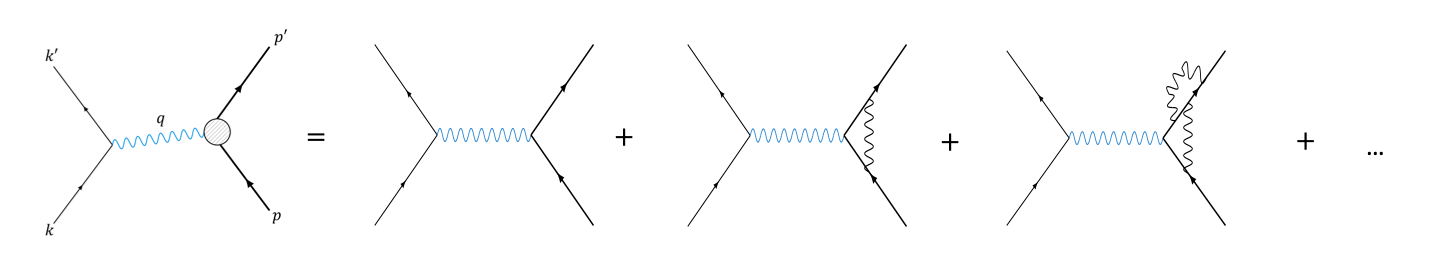
\includegraphics[width=\linewidth]{figures/feyn_sum.png}
	\caption{The contributions of higher order diagrams.}
	\label{fig:feyn_sum}
\end{figure}

The scattering probability amplitude cannot be known exactly because of the processes beyond the first order (tree level) that could occur in Fig. \ref{fig:feyn_epscatt} at the proton-$\gamma^{*}$ vertex blob (these contributions can be seen in Fig. \ref{fig:feyn_sum}). However, we can handle the mathematical description of these processes by expressing the scattering probability amplitude matrix in terms of the leptonic and hadronic tensors
\begin{equation}
\label{eqn:el_M2}
|\mathcal{M}|^2 = \frac{e^4}{Q^4} \ell_{\mu\nu} W^{\mu \nu}.
\end{equation}
The leptonic tensor $\ell_{\mu\nu}$ is associated with the coupling of the virtual photon to the electron (more generally the coupling of the exchange boson to the lepton), and for unpolarized scattering can be expressed as
\begin{equation}
\label{eqn:lep_tens}
\ell_{\mu\nu} = \bar{u}(k',s')\gamma^{\mu}u(k,s) \bar{u}(k,s) \gamma^{\nu} u(k',s').
\end{equation}
The term $u(k)$ is the Dirac spinor. For the electron (a spin-$1/2$ fermion), there are two spin states ($i.e.$ up or down) so there are two associated spinors that could exist here
\begin{equation}
u_{\uparrow}(k) = \left( \begin{array}{c} 1 \\ 0 \\ \frac{k_z}{E+m} \\ \frac{k_x+ik_y}{E+m} \end{array} \right) \; \; \mathrm{and} \; \;
u_{\downarrow}(k) = \left( \begin{array}{c} 0 \\ 1 \\ \frac{k_x-ik_y}{E+m} \\ \frac{-k_z}{E+m} \end{array} \right),
\end{equation}
where $m$ is the lepton mass, $k_{x,y,z}$ are the momentum components of the initial lepton. In Eq. \ref{eqn:lep_tens}, $\gamma^{\mu}$ are the gamma matrices. When summed and averaged over spins, the leptonic tensor (following \cite{book:bjorken_drell,}) becomes
\begin{eqnarray}
\nonumber
\ell_{\mu\nu} &=& \mathrm{Tr} \left[ \frac{\slashed{k}'+m}{2m} \gamma^{\mu} \frac{\slashed{k}+m}{2m} \gamma^{\nu} \right] \\
\nonumber
&=& \frac{1}{m^2} \mathrm{Tr} (\slashed{k}'\gamma^{\mu}\slashed{k}\gamma^{\nu} + m^2\gamma^{\mu}\gamma^{\nu}) \\
&=& 2 (k'^{\mu}k^{\nu} + k^{\mu}k'^{\nu} - g^{\mu\nu}k' \cdot k).
\end{eqnarray}
Thus far we have from Eq. \ref{eqn:el_M2}
\begin{equation}
|\mathcal{M}|^2 = \frac{e^4}{Q^4} 2 (k'^{\mu}k^{\nu} + k^{\mu}k'^{\nu} - g^{\mu\nu}k' \cdot k) W^{\mu \nu},
\end{equation}
where $g^{\mu\nu}$ is the metric tensor.

We must now take a look at the hadronic tensor $W^{\mu\nu}$, which is more complicated because we must take into account the proton's structure. In fact, the hadronic tensor cannot be known exactly. It can, however, be expanded to the second order as
\begin{equation}
W^{\mu\nu} = \bra{p}J^{\nu}\ket{p'}\bra{p'}J^{\mu}\ket{p},
\end{equation}
which depends on the $J^{\mu}$ current matrix elements. That current between two nucleon states (following \cite{book:halzen})
\begin{equation}
\bra{p}J^{\mu}(0)\ket{p'} = \bar{U}(p')\left[ F_1(Q^2)\gamma^{\mu}+F_2(Q^2)\frac{i\sigma^{\mu\nu}}{2M_N} \right]U(p)
\end{equation}
gives rise to two form factors, $F_1(Q^2)$ which is called the Dirac form factor and $F_2(Q^2)$ called the Pauli form factor. Here $\sigma^{\mu\nu}=\tfrac{i}{2}[\gamma^{\mu},\gamma^{\nu}]$ and we denote the difference between the lower-case $u(k,s)$ electron spinors from Eq. \ref{eqn:lep_tens} and upper-case $U(p)$ nucleon spinors. If we introduce the more physically interesting Sach's electric and magnetic form factors respectively
\begin{equation}
\nonumber
G_E(Q^2) = F_1(Q^2) + \frac{Q^2}{4M_N^2} F_2(Q^2)
\end{equation}
\begin{equation}
\nonumber
G_M(Q^2) = F_1(Q^2) + F_2(Q^2),
\end{equation}
then the hadronic tensor can be written as
\begin{eqnarray}
\nonumber
W^{\mu\nu} &=& 2(p'^{\mu}p^{\nu} + p'^{\nu}p^{\mu} - g^{\mu\nu}(pp'-M_N^2))G_M^2 \\
\nonumber
&&- 2F_2G_M(p+p')^{\mu}(p+p')^{\nu}+F_2^2\frac{M_N^2+p \cdot p'}{2M_N^2}(p+p')^{\mu}(p+p')^{\nu} \\
\nonumber
&=& (-q^{\mu}q^{\nu}+g^{\mu\nu}q^2)G_M^2+(p+p')^{\mu}(p+p')^{\nu}\frac{G_E^2+\tau G_M^2}{1+\tau} \\
&=& g^{\mu\nu}q^2G_M^2+4p^{\mu}p^{\nu}\frac{G_E^2+\tau G_M^2}{1+\tau} + ...,
\end{eqnarray} 
where we define $\tau = Q^2/4M_N^2$ to simplify the expression. Because of current conservation, the terms containing factors of $q^{\mu}$ are omitted with the ellipses, since they do not contribute to the cross section.

Substituting our expressions for the leptonic and hadronic tensors for elastic scattering in the lab frame and contracting them, we arrive at
\begin{equation}
\label{eqn:el_cs}
\frac{d\sigma}{d\Omega} = \left( \frac{d\sigma}{d\Omega} \right)_{\mathrm{Mott}} f_{\mathrm{rec}} \left[ \frac{G_E^2(Q^2) + \tau G_M^2(Q^2)}{1+\tau} + 2\tau G_M^2 \tan \frac{\theta}{2} \right],
\end{equation}
where $\left( \tfrac{\mathrm{d}\sigma}{\mathrm{d}\Omega} \right)_{\mathrm{Mott}}$ comes from Eq. \ref{eqn:mott} ($i.e.$ the Mott cross section) and $f_{\mathrm{rec}}$ is the recoil factor equal here to $E'/E$. As $Q^2$ gets very high, $\tau$ increases and the magnetic form factor $G_M(Q^2)$ dominates. Eq. \ref{eqn:el_cs} gives a more physical description of the elastic scattering cross section in terms of kinematic variables that can be measured through scattering experiments.

One more kinematic variable that needs to be introduced offers insight into cases when scattering enters into inelastic regimes. The invariant mass squared $W^2$ (not to be confused with the hadronic tensor $W^{\mu\nu}$) of the photon-nucleon system, is defined mathematically as 
\begin{equation}
W^2 = (q+p)^2 =M_N^2 + 2M_N\nu - Q^2,
\end{equation}
where $\nu = E-E'$ is the energy transfered from the electron to the nucleon via virtual photon ($\gamma^*$). In the elastic scattering case , $W^2 = M_N^2$, because $Q^2$ and thus $\nu$ are small ($i.e.$ $E << M_N$). As $Q^2$ increases, instead of simply bouncing off of the nucleon, the energy transfered to the nucleon begins changing the state of the quarks within the nucleon. 

\section{Resonance Region}
Changing the state of a quark within the nucleon results in excited states of that nucleon, called \textit{resonances}. The region where resonances occur is $M_N^2 < W^2 < 4 \; \mathrm{GeV}^2$, and is called the \textit{resonance region}. There are 6 families of resonances that depend on the characteristics of the resonant particles. Particles containing only $u$ and $d$ quarks, whose isospin $I= \tfrac{1}{2}$, are denoted by $N$. The $\Delta$ family of resonances also have only $u$ and $d$ quarks, but have $\tfrac{3}{2}$ isospin. When $I=0$ and the particle contains $u$, $d$ and one $c$, $s$, or $b$ quark, it is called a $\Lambda$ resonance. The $\Sigma$ resonance also has $u$, $d$ plus one $c$, $s$, or $b$ quark, but with $I=1$. When only one $u$ or $d$ quark exists with two $c$, $s$, or $b$ quarks with $I=\tfrac{1}{2}$, it is a $\Xi$ resonance. Finally, when $I=0$ and only $c$, $s$, or $b$ quarks are present, it is known as an $\Omega$ resonance\cite{PDG}.

Unlike the ground state of nucleons, these excited states are extremely short lived (on the order of $10^{-23}$ seconds). After their short life, these resonances decay into more stable hadrons. Detection of the these hadrons is what provides proof of the existence of resonant states. For example, a common resonance $\Delta^0(1232)$, which is the lowest lying resonance with a mass of $1.232$ GeV\cite{PDG}, predominately decays via the strong interaction into a pion ($\pi^0$) and a neutron ($n$) or to $\pi^-p$. The entire interaction begins at the first step of creating an excited state
\begin{equation}
p+e^- \longrightarrow \Delta^0 + e'
\end{equation}
then decays into
\begin{equation}
\Delta^0 \longrightarrow \pi^0 + n.
\end{equation}
However, because these resonances are so short-lived, it is convention to express the entire interaction as
\begin{equation}
\nonumber
p+e^- \longrightarrow e'^- + \pi^0 + n.
\end{equation}
\begin{equation}
\label{eqn:delta_res}
p+e^- \longrightarrow e'^- + \pi^- + p.
\end{equation}
One reason for this convention is that there are many resonances that can produce the same final state($i.e.$ $\pi^0$ and $n$ in our example). Knowing exactly what resonance produced a particular final state can be difficult. In the example of Eq. \ref{eqn:delta_res}, the $\Delta^0$ has the same quark makeup as the neutron ($i.e.$ $udd$), but is much heavier. Measuring the invariant mass of the resulting particles is one of the few ways to understand what resonance occurred. 

Similar to elastic scattering, interactions with resonances can be described using form factors. The analogous cross section (following the treatment of \cite{stoler}) is
\begin{equation}
\frac{d\sigma}{d\Omega} = \left( \frac{d\sigma}{d\Omega} \right)_{\mathrm{Mott}} f_{\mathrm{rec}} \left( \frac{|G_E|^2+\tau^*|G_T|^2}{1+\tau^*} + 2\tau^* |G_T|^2 \tan^2 \frac{\theta}{2} \right) R(W),
\end{equation}
where $f_{\mathrm{rec}}$ is the recoil factor of the proton, $\tau^*$ is the analogous kinematic quantity of $\tau$ from elastic scattering, $G_E$ and $G_T$ are the resonance longitudinal and transverse form-factors respectively, and $R(W)$ is called the resonance line shape. In inelastic scattering of resonances
\begin{equation}
f_{\mathrm{rec}} = \frac{E'}{E} \left[ \frac{1}{1-\frac{(W_R^2 - M_N^2)}{2M_NE}} \right],
\end{equation}
and
\begin{equation}
R(W) = \frac{2\pi^{-1}W_R M_N \Gamma_R}{(W^2-W_R^2)^2 + W_R^2 \Gamma_R^2}.
\end{equation}
The quantities $W_R$ and $\Gamma_R$ refer to the resonance mass and width respectively. If the resonance width is small enough ($i.e.$ when $W_R=M_N$ and $W_R \Gamma_R \rightarrow 0$), $R(W)$ becomes a $\delta$-function and the resonance cross section reduces to that of an elastic cross section. 

At low $Q^2$, we can describe interactions by constituent quarks models. At high $Q^2$ we enter a region best described with perturbative quantum chromodynamics (pQCD). We will discuss more about pQCD in a later section. The resonance region is an important bridge between these two regimes. Determining resonance form factors allows us to describe the resonance transition the same way elastic form factors describe elastic interactions.

\section{Deep Inelastic Scattering}
Once the energy transfered to the nucleon ($Q^2$) becomes large enough, the probability of creating excited (resonance) states decreases and there becomes a higher probability of the virtual photon ``elastically" scattering off a quark inside the nucleon. This is known as \textit{deep} inelastic scattering. This happens at roughly $W > 2$ MeV and $Q^2 > 1$ $\mathrm{GeV}^2$.. In this regime we can probe the inner structure of the nucleon. 

\begin{figure}[h!]
	\centering
	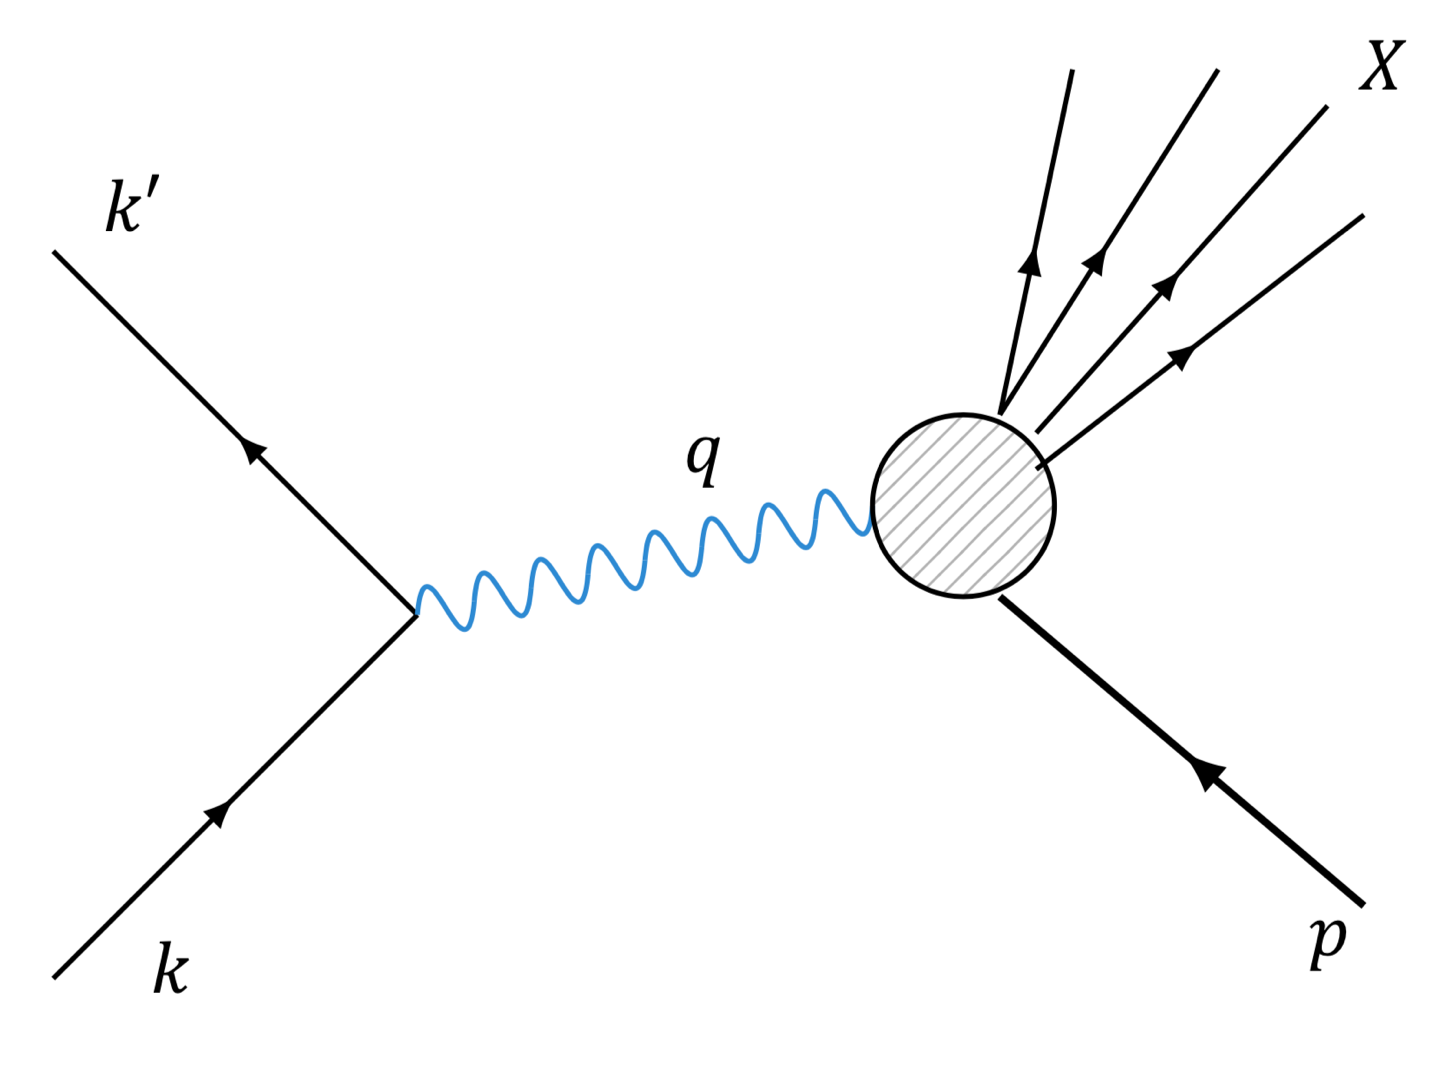
\includegraphics[width=0.6\linewidth]{figures/feyn_inelscatt.png}
	\caption{Feynman diagram of deep inelastic electron scattering from a proton.}
	\label{fig:feyn_inelscatt}
\end{figure}

However, because the energy transfer is so high, the proton often breaks apart in the interaction
\begin{equation}
ep \longrightarrow e'X,
\end{equation}
where $X$ denotes all possible particles that might emerge from the proton-electron collision. The Feynman diagram also must be altered from Fig. \ref{fig:feyn_epscatt} to Fig. \ref{fig:feyn_inelscatt}, where $X$ again represents all possible emerging particles. The deep-inelastic scattering cross section can be written (following \cite{book:halzen}) as
\begin{equation}
\frac{d^2\sigma}{dE'\Omega} = \frac{4\alpha^2E'^2}{q^4} \left[ W_2(\nu,Q^2)\cos^2\frac{\theta}{2} +2W_1(\nu,Q^2) \sin^2 \frac{\theta}{2} \right],
\end{equation}
where $W_1$ and $W_2$ are called inelastic structure functions. These structure functions are the analogs to the form factors in Eq. \ref{eqn:el_cs} for elastic scattering. There is much more to discuss about deep-inelastic scattering, but first we must discuss how to treat scattering off quarks (or more broadly, partons) within a nucleon with an approach called \textit{scaling}.

\section{Partons and Bjorken-Scaling}
The way we probe inside nucleons is with the exchange of small wavelength (large $Q^2$) virtual photons, which interacts with partons inside the nucleon. This can be handled using the inelastic structure functions $W_1$ and $W_2$, which are functions of the energy lost by the electron due to nucleon recoil ($i.e.$ $\nu$) and the negative four-momentum squared of the virtual photon ($i.e.$ $Q^2$). When the virtual photon has a small enough wavelength (large enough $Q^2$), the nucleon that was once described by Eq. \ref{eqn:el_cs} starts to look more like a free Dirac particle and the cross section (following \cite{book:halzen}) becomes
\begin{equation}
\label{eqn:quark_scatt}
\frac{d\sigma}{dE'd\Omega} = \frac{4 \alpha^2 e_q^2 E'^2}{q^4} \left( \cos^2 \frac{\theta}{2} - \frac{q^2}{2m^2}\sin^2 \frac{\theta}{2} \right) \delta \left( \nu + \frac{q^2}{2m} \right).
\end{equation} 
Remarkably, this is the equation for the electron elastic scattering cross section from a structureless particle\cite{book:halzen}. Here $e_q$ is the fractional charge of that structureless particle and $m$ is that particle's mass. This particle inside the nucleon was eventually called a quark.

\begin{figure}[h!]
	\centering
	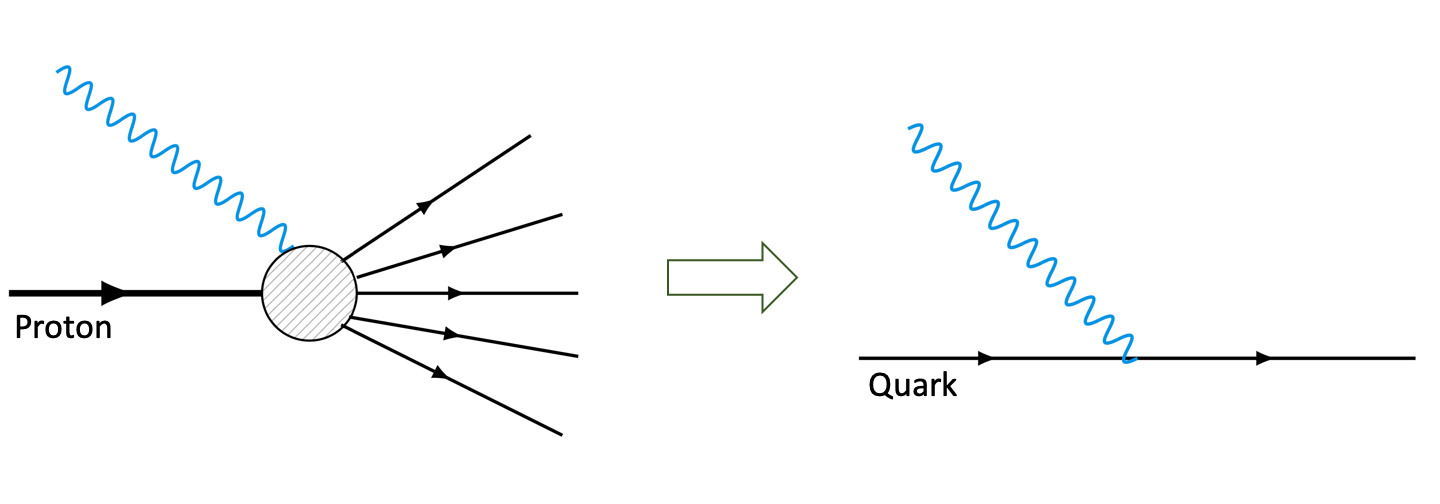
\includegraphics[width=0.9\linewidth]{figures/inel_to_dis.png}
	\caption{The transition from inelastic scattering to deep inelastic scattering of a virtual photon and the quark within a nucleon.}
	\label{fig:feyn_inel_to_dis}
\end{figure}

In this case, where the virtual photon elastically scatters off of a quark within the nucleon described by Eq. \ref{eqn:quark_scatt}, the nucleon structure functions become
\begin{equation}
\label{eqn:dis_sf_1}
2W_1^{\mathrm{point}} = \frac{Q^2}{2m^2} \delta \left( \nu - \frac{Q^2}{2m} \right)
\end{equation}
and
\begin{equation}
\label{eqn:dis_sf_2}
W_2^{\mathrm{point}} = \delta \left( \nu - \frac{Q^2}{2m} \right).
\end{equation}
Here, thus in Eq. \ref{eqn:quark_scatt}, there exists the delta function that conserves energy in the interaction. Fig. \ref{fig:feyn_inel_to_dis} shows the resulting diagram when we take the right side of Fig. \ref{fig:feyn_inelscatt} (the left side of Fig. \ref{fig:feyn_inel_to_dis}) and begin to probe a single quark inside the nucleon (the right side of Fig. \ref{fig:feyn_inel_to_dis}). This reduction is representative of the electron elastically scattering off a quark in the nucleon.

If we take Eq. \ref{eqn:dis_sf_1} and \ref{eqn:dis_sf_2}, using the identity $\delta(x/a) = a\delta(x)$, we can write
\begin{equation}
\nonumber
2mW_1^{\mathrm{point}}(\nu,Q^2) = \frac{Q^2}{2m\nu} \delta \left( 1- \frac{Q^2}{2m\nu} \right)
\end{equation}
\begin{equation}
\nu W_2^{\mathrm{point}}(\nu,Q^2) = \delta \left( 1- \frac{Q^2}{2m\nu} \right).
\end{equation}
These equations for the structure functions are now dimensionless and depend on only the ratio $Q^2/2m\nu$, which is both important and useful. That usefulness is as follows: when $Q^2$ is high enough, the virtual photon begins to elastically scatter off of structureless (point) particles  within the nucleon and can be described using the dimensionless structure functions
\begin{equation}
\nonumber
MW_1(\nu,Q^2) \xrightarrow[\text{large $Q^2$}]{} F_1(x_B)
\end{equation}
\begin{equation}
\nu W_2(\nu,Q^2) \xrightarrow[\text{large $Q^2$}]{} F_2(x_B).
\end{equation}
Here $x_B$ is introduced as the Bjorken-$x$ scaling variable defined as
\begin{equation}
x_B = \frac{Q^2}{2M\nu},
\end{equation}
which describes the momentum fraction of a quark or gluon within a nucleon. Up to this point, we have only discussed interactions between the virtual photon and the quarks within the nucleon, but that virtual photon can also interact with gluons that exists in the nucleon. Collectively, these quarks and gluons in the nucleon are known as partons. The Bjorken-$x$ scaling variable can describe the momentum fraction of any parton within a nucleon.

The relationship between the structure functions $F_1(x_B)$ and $F_2(x_B)$ (known as the Callan-Gross relation) is
\begin{equation}
2x_B F_1(x_B) = F_2(x_B) = \sum_i e_i^2 f_i (x_B). 
\end{equation} 
In the right side of this expression we have a sum over partons (the parton index is $i$) of the square of that parton's charge ($e_i^2$) times $f_i(x_B)$, known at the parton distribution function. The parton distribution function (or PDF) 
\begin{equation}
f_i(x_B) = \frac{dP_i}{dx_B},
\end{equation}
describes the probability $P_i$ that a struck parton $i$ carries a fraction ($x_B$) of the nucleon's momentum.

Because $F_2(x_B)$ offers a straightforward interpretation in terms of quarks, the $F_2$ structure function is the more important term here to examine experimentally and is of interest in the BONuS12 Experiment. For deep-inelastic electron-proton scattering, the $F_2^p(x_B)$ structure function is
\begin{eqnarray}
\label{eqn:F_p}
\frac{1}{x_B} F_2^p(x_B) &=& \left( \frac{2}{3} \right)^2 [u^p(x_B)+\bar{u}^p(x_B)] + \left( \frac{1}{3} \right)^2 [d^p(x_B)+\bar{d}^p(x_B)] \\
&& + \left( \frac{1}{3} \right)^2 [s^p(x_B)+\bar{s}^p(x_B)],
\end{eqnarray}
where $p$ superscript denotes that we are dealing with the proton structure, and the PDF $f_i(x_B)$ is replaced with the first letter of the quark name ($e.g.$ the up quark and antiquark PDF's are denoted as $u^p(x_B)$ and $\bar{u}^p(x_B)$ respectively). The contributions of quarks heavier than the strange quark have been assumed to be negligible here. The neutron structure function $F_2^n(x)$, where we have dropped the $B$ in $x_B$, is
\begin{eqnarray}
\label{eqn:F_n}
\frac{1}{x} F_2^n(x) &=& \left( \frac{2}{3} \right)^2 [u^n(x)+\bar{u}^n(x)] + \left( \frac{1}{3} \right)^2 [d^n(x)+\bar{d}^n(x)] \\
&& + \left( \frac{1}{3} \right)^2 [s^n(x)+\bar{s}^n(x)].
\end{eqnarray}
This looks similar to the $F_2^p$ structure function because the proton and neutron are together part of an isospin doublet. When particles are members of an isospin doublet, they can transform into each other under an $SU(2)$ transformation
\begin{equation*}
\begin{pmatrix}
p \\ n 
\end{pmatrix}
\xrightarrow[\text{$SU(2)$}]{}
\exp \left( -\frac{i}{2}\theta_a \sigma_a \right)
\begin{pmatrix}
p \\ n
\end{pmatrix},
\end{equation*}
where $p$ and $n$ are proton and neutron states, and $\sigma_a$ are the Pauli matrices. This transformation means that the quark contents of the proton and neutron are related.

\section{Nucleon Structure-Function Ratio $F^2_n/F^2_p$}
We can exploit this relation between quark contents of protons and neutrons to study the structure of nucleons, in particular the neutron structure. That relationship between quark contents means
\begin{eqnarray}
\nonumber
u^p(x) &=& d^n(x) \equiv u(x), \\
d^p(x) &=& u^n(x) \equiv d(x), \\
\nonumber
s^p(x) &=& s^n(x) \equiv s(x). \\
\end{eqnarray}
The probability of finding a $u$ quark in a proton is the same as the probability of finding a $d$ quark in a neutron. Each nucleon consists not only of $u_v$ and $d_v$ quarks that determine the quantum numbers of the nucleon (called \textit{valence} quarks, hence the subscript $v$), but many quark-antiquark pairs in a constant state of creation and annihilation (known as \textit{sea} quarks). In the first order approximation, we can assume that the lighter quark-antiquark pairs $u_s\bar{u}_s$, $d_s\bar{d}_s$, and $s_s\bar{s}_s$ contribute to this ``sea" and we can neglect contributions from the heavier quark-antiquark pairs $c_s\bar{c}_s$ and so on.

\begin{figure}[h!]
	\centering
	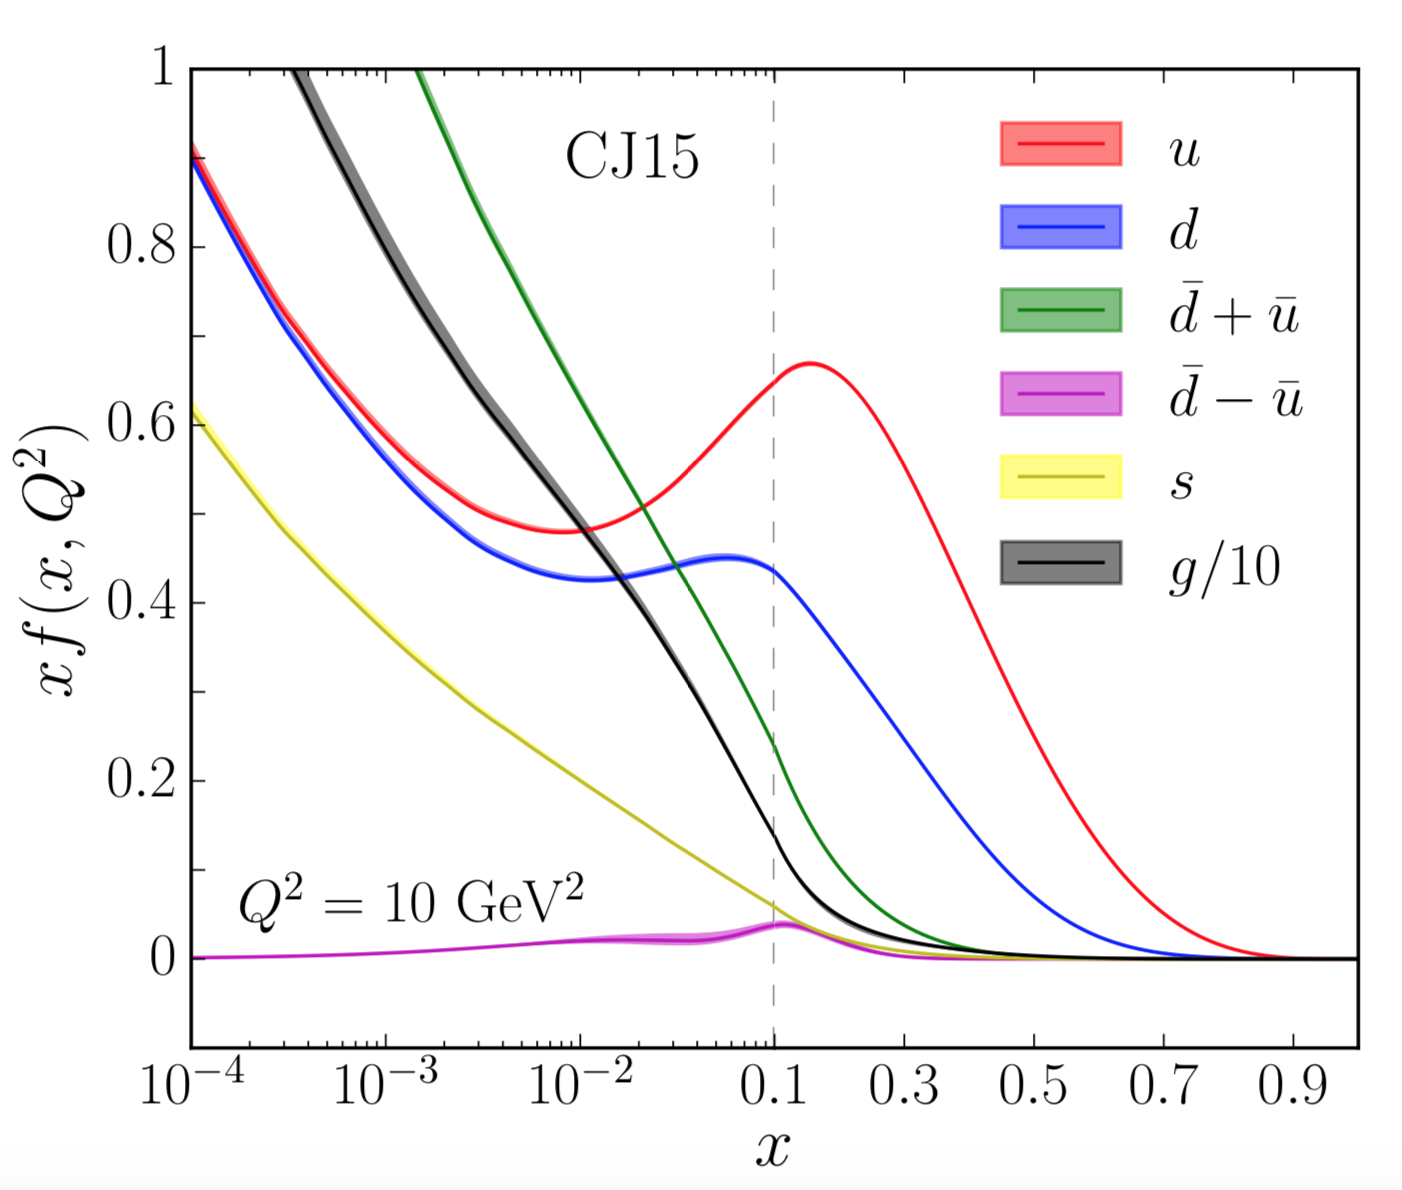
\includegraphics[width=0.9\linewidth]{figures/xf_x.png}
	\caption{Comparison of CJ15 PDFs $xf(x,Q2)$ for different flavors ($f = u, d, \bar{d}+\bar{u}, \bar{d}−\bar{u}, s$ and $g/10$) at a scale $Q^2 = 10$ GeV$^2$, with 90\% CL uncertainty bands. Note the combined logarithimic/linear scale along the x-axis.\cite{CJ15}}
	\label{fig:xf_x}
\end{figure}

This approximation of the nucleon structure results in adding the sea quarks to the contributions of each quark type. That is
\begin{eqnarray}
\nonumber
u(x) &=& u_v(x) + u_s(x), \\
d(x) &=& d_v(x) + d_s(x), \\
u_s(x) &=& \bar{u}_s(x) = d_s(x) = \bar{d}_s(x) = s_s(x) = \bar{s}_s(x) = S(x),
\end{eqnarray}
where we now use $S(x)$ for all sea quark contributions. If we combine this relationship with our expressions for the proton and neutron structure functions Eqs. \ref{eqn:F_p} and \ref{eqn:F_n}, respectively, we get
\begin{equation}
\frac{1}{x} F_2^p = \frac{1}{9}[4u_v + d_v] + \frac{4}{3} S
\end{equation}
and 
\begin{equation}
\frac{1}{x} F_2^n = \frac{1}{9}[u_v + 4d_v] + \frac{4}{3} S,
\end{equation}
where the $\tfrac{4}{3}$ comes from summing over all six sea quark distributions. In the low $x$ limit ($i.e.$ $x \rightarrow 0$), the ratio of $F_n^2/F_2^p$ goes to unity, or

\begin{equation}
\frac{F_2^n}{F_2^p} \xrightarrow[\text{$x \rightarrow 0$}]{} 1.
\end{equation}
However, as we approach $x \rightarrow 1$ that ration becomes
\begin{equation}
\label{eqn:f2n_f2p}
\frac{F_2^n}{F_2^p} \xrightarrow[\text{$x \rightarrow 1$}]{} \frac{u+4d}{4u+d},
\end{equation}
where $u$ and $d$ are the valance $up$ and $down$ quarks and $S\rightarrow0$. We can see in Fig. \ref{fig:xf_x} that as $x>0.3$, the $u$ and $d$ quarks dominate, so Eq. \ref{eqn:f2n_f2p} neglects the sea-quark contributions as well as $strange$ and larger mass sea-quark contributions. We can rearrange Eq. \ref{eqn:f2n_f2p} to get the $d/u$ ratio
\begin{equation}
\label{eqn:d/u}
\frac{d}{u} \approx \frac{4F_2^n/F_2^p-1}{4 - F_2^n/F_2^p},
\end{equation}
which provides important insight into the parameterizations of PDFs at large $x$.

\section{Models and Predictions}
If SU(6) symmetry were exact, then the $u$ and $d$ quarks within the proton would be identical with the exceptions of charge and flavor. The wave function of a proton polarized in the $+z$ direction \cite{book:close}  would be
\begin{eqnarray}
\label{eqn:pol_p}
\nonumber
p \uparrow &=& \frac{1}{2}u\uparrow(ud)_{S=0} + \frac{1}{\sqrt{18}}u\uparrow (ud)_{S=1} - \frac{1}{3}u\downarrow(ud)_{S=1} \\
&&- \frac{1}{3}d\uparrow(uu)_{S=1} - \frac{\sqrt{2}}{3}d\downarrow(uu)_{S=1},
\end{eqnarray}
where the subscript are the spins of the diquark pairs. The quark distribution in this case would be the same for both $u$ and $d$ quarks, which implies $u=2d$ for all $x$. This leads to the $F_2$ structure function and $d/u$ ratios
\begin{equation}
\frac{F_2^n}{F_2^p}  = \frac{2}{3}, \; \; \frac{d}{u} = \frac{1}{2}.
\end{equation}
This is known as the SU(6) quark model. This symmetry, however, is broken in nature as there is a nonzero difference between quark masses as well as a measured value of the $F_2^n/F_2^p$ ratio far below $2/3$.

There are a few explanations out there for SU(6) symmetry breaking. Close \cite{physrep:close} and Cartlitz \cite{physrep:carlitz} observed the correlation between large-$x$ behavior of $F_2^n/F_2^p$ and the mass splitting of the nucleon and $\Delta$ baryons. They assumed that the stuck nucleon breaks into a single quark which interacts with the virtual photon and a diquark pair. When $x \rightarrow 1$, the $S=1$ state term becomes small compared to the $S=0$ state term. This suppression of the $S=1$ diquark state can explain the symmetry breaking and leads to the first term in Eq. \ref{eqn:pol_p} to dominating. Therefore at $x\approx 1$, $F_2^p$ is essentially given by the single $u$ quark distribution and so
\begin{equation}
\frac{F_2^n}{F_2^p}  = \frac{1}{4}, \; \; \frac{d}{u} =0.
\end{equation}
Isgur \cite{physrep:insgur1} \cite{physrep:insgur2} describes this $d$-quark suppression by a color hyperfine interaction arising from a one-gluon exchange. In the lowest order, the Hamiltonian of the hyperfine-perturbed quark model for the color-magnetic hyperfine interaction between two quarks is proportional to $S_i \cdot S_j$, where $S_i$ is the spin vector of quark $i$. This means that if the spins are parallel, the force is repulsive, and if the spins are anti-parallel then the force is attractive. Therefore, $S=1$ is suppressed and $d/u =0$ as $x \rightarrow 1$.

\begin{figure}[h!]
	\centering
	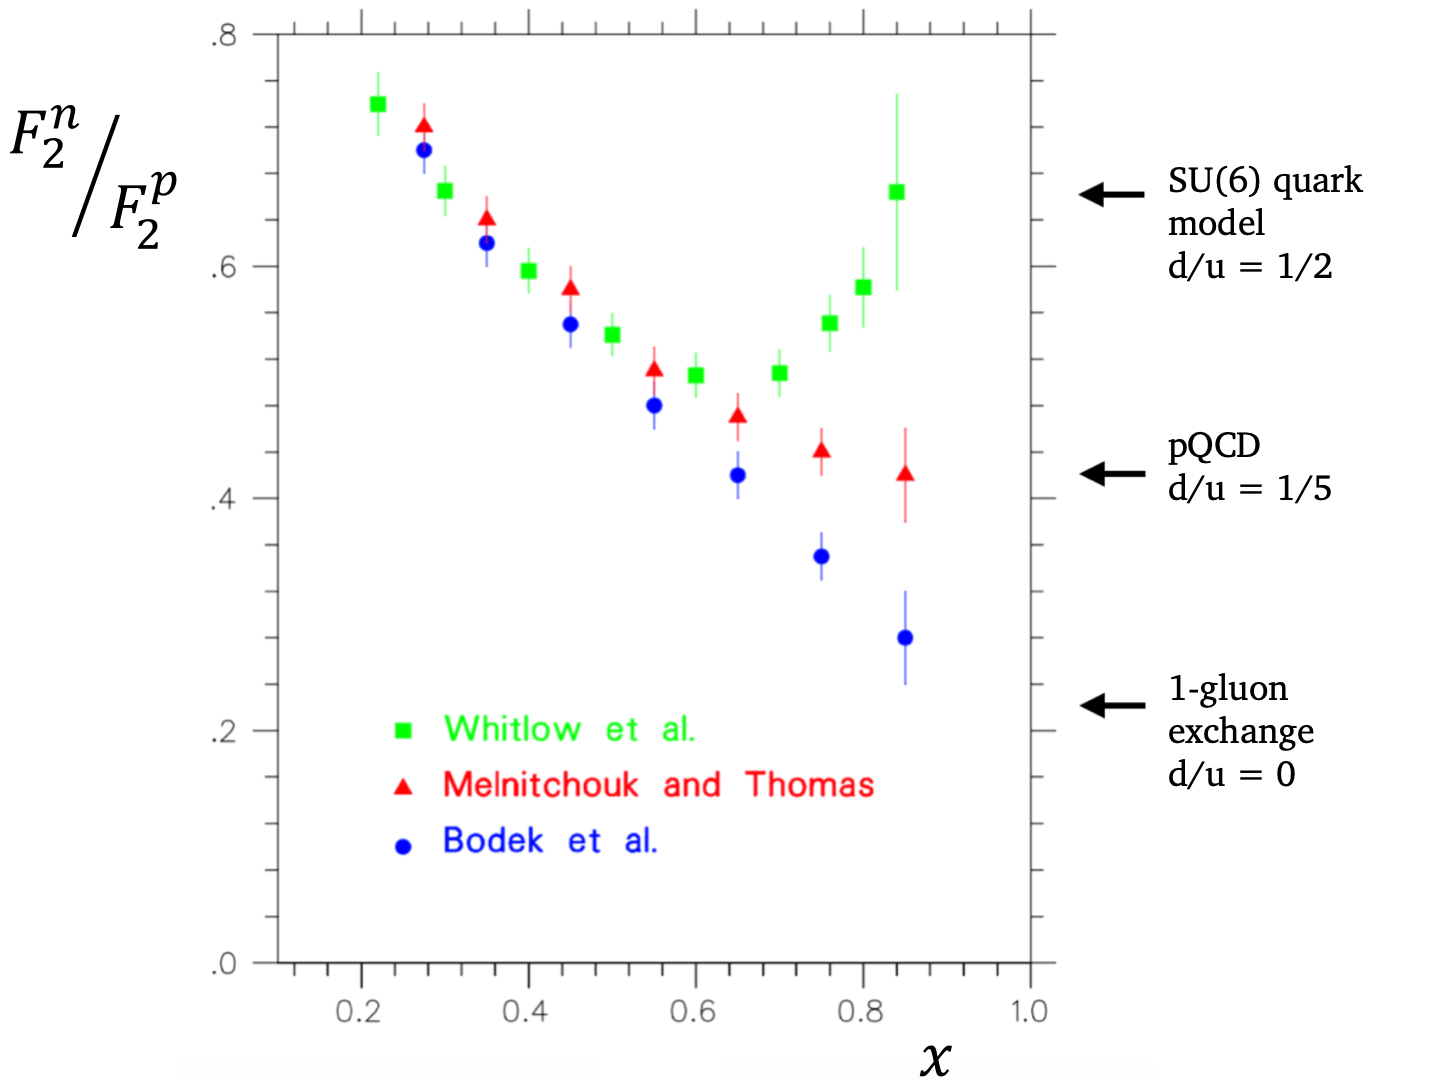
\includegraphics[width=0.9\linewidth]{figures/f2n_f2p_models.png}
	\caption{Model dependence of $F_2^n/F_2^p$. \cite{marathon}}
	\label{fig:f2n_f2p_models}
\end{figure}

The last model that will be introduced here that proposed to explain the SU(6) symmetry breaking is based on perturbative QCD first from Farrar and Jackson \cite{physlett:farrar}. They put forward that at $x \approx 1$, the hadronic structure functions could be calculated to the lowest order perturbation theory to $O(m^2/q^2)$, where the incoming quarks could be thought of as ``free". The valence quark wave function that dominates here is the diquark spin projection $S_z = 0$. When the spins of two quarks are aligned, scattering is suppressed by a factor of ($1-x$) less than anti-aligned quarks. That is, $S_z = 0$ diquark states dominate when $x \rightarrow 1$. The $u$ quark having the same helicity as the proton is 5 times as likely as the $d$ having the same helicity as the proton. This results in
\begin{equation}
\frac{F_2^n}{F_2^p}  = \frac{3}{7}, \; \; \frac{d}{u} =\frac{1}{5}.
\end{equation}
More recently, Brodsky \cite{brodsky} used a hard gluon exchange model based on quark counting rules leading to the same conclusion.
 
 \begin{figure}[h!]
 	\centering
 	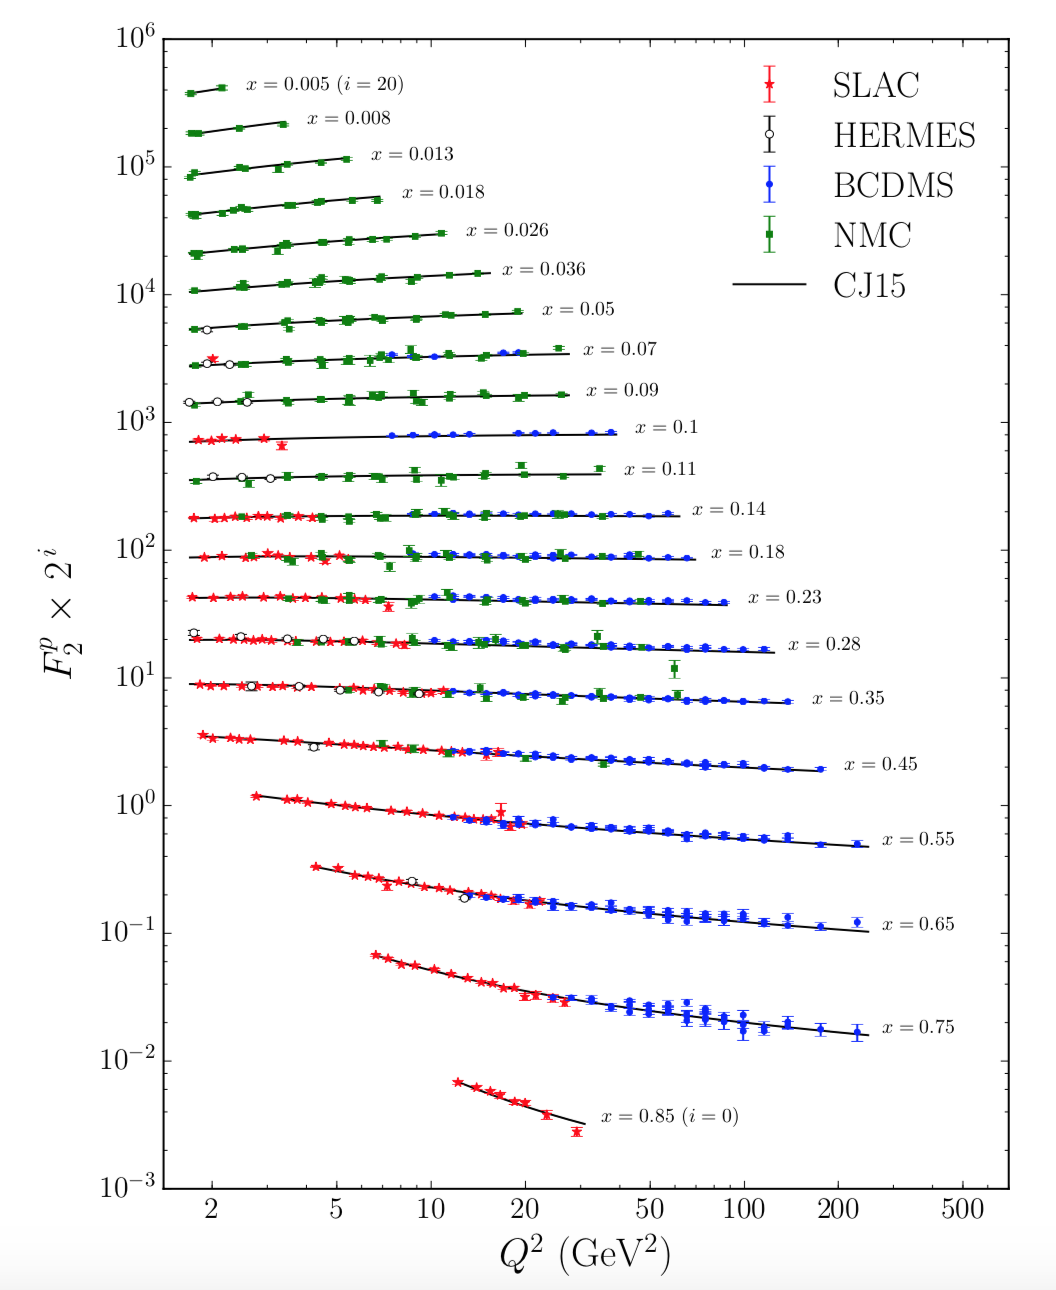
\includegraphics[width=0.9\linewidth]{figures/F2p.png}
 	\caption{Measured values of $F_2^p$ vs $Q^2$ for different values of $x$. \cite{CJ15}}
 	\label{fig:f2p}
 \end{figure}
 
All of these predictions can be summarized in Fig. \ref{fig:f2n_f2p_models}, which makes it obvious that the value of $F_2^n/F_2^p$ is very much model dependent. It is the goal of the BONuS12 experiment to measure this ratio in a model independent way. In order to do this, we need to know the values of both $F_2^p$ and $F_2^n$ to high precision. Much is known about the $F_2^p$ structure function because it can be extracted from electron scattering from protons in hydrogen targets. Fig. \ref{fig:f2p} shows the multiple experiments and kinematic ranges where $F_2^p$ has been measured. The trouble with Eq. \ref{eqn:f2n_f2p} and Eq. \ref{eqn:d/u} is our knowledge of the $F_2^n$ structure function.

\section{Difficulties in Extracting $F_2^n/F_2^p$ from Deuterium}
There are no free neutron targets to conduct scattering experiments from like there is for protons in hydrogen targets. Free neutrons decay in about 15 minutes and are electrically neutral, which means they cannot be confined using magnets. Therefore, the $F_2^n$ structure function must be extracted from scattering experiments using targets like Helium-3 (two protons and a neutron), Helium-4 (two protons and two neutrons), and deuterium (one proton and one neutron). The BONuS12 Experiment uses a deuterium target.

\begin{figure}[h!]
	\centering
	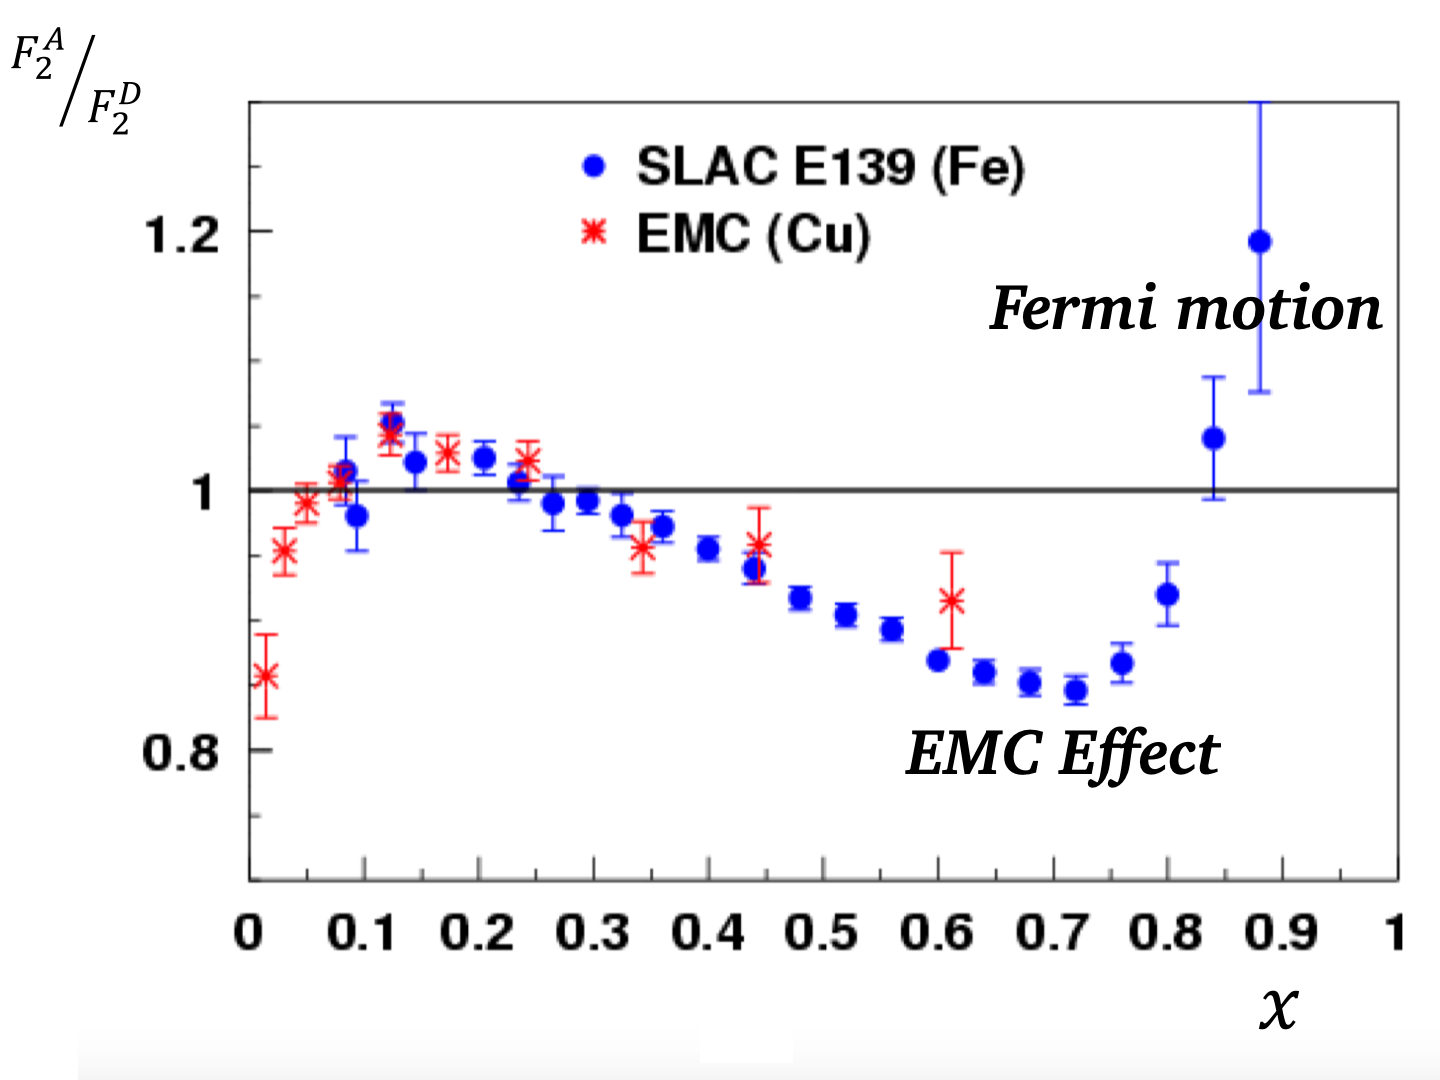
\includegraphics[width=0.9\linewidth]{figures/EMC.png}
	\caption{Variations of the $F_2^A/F_2^D$ ratio from unity indicating various nuclear binding effects. \cite{emc1}\cite{emc2}}
	\label{fig:emc}
\end{figure}

The trouble with using any nuclear target with two or more nucleons to study the structure of a single nucleon is that those nucleons do no behave as they do when they are free. Early DIS experiments by the Electron Muon Collaboration (EMC) in CERN found that the ratio $F_2^A/F_2^D$ (superscript $A$ denotes the mass number of a nuclear target and $D$ denotes deuterium) was not unity for all values of $x$. Fig. \ref{fig:emc} shows that deviation for experiments done on iron and copper nuclei. This deviation indicates that quark distributions are different for free and bound nucleons.

Because the EMC first discovered this phenomena, the deviation between $0.2<x<0.8$ was dubbed the EMC effect. The other contributors are known as shadowing ($x<0.1$), anti-shadowing ($0.1<x<0.2$) and $x>0.8$ is believed to be due to Fermi motion. Just like partons in a nucleon, nucleons in a nucleus are not stationary. Fermi motion refers to the motion of nucleons within a nucleus.

There are many models attempting to explain the EMC effect (for a detailed review, see \cite{emc_rev}), but none have been proven experimentally. The EMC effect is not proportional to $A$ (this was proven with scattering from $^4$He) or average nuclear density (ruled out by scattering from $^9$Be). However, a model of $Q^2$ rescaling pointing to increased quark confinement, which could explain the EMC effect\cite{emc_rev}.

\section{Spectator Tagging}
The goal of the BONuS12 Experiment and other experiments concerned with measuring the structure of neutrons is to do so without significant model dependence at high-$x$ or involvement of bound-nucleon issues. To do this effectively, since the neutron of interest is bound within a nucleus, BONuS12 uses a method called spectator tagging. In particular, since the electron ($e$) is meant to scatter from the neutron within deuterium ($D$) in the interaction
\begin{equation}
\label{eqn:eD_epX}
eD \longrightarrow e'p_s X,
\end{equation}
the proton ($p_s$) needs to be a spectator to the reaction. That is, the proton plays no role in the interaction, thereby not interacting with any of the debris ($X$) coming from the struck neutron.

The cross section of the reaction given in Eq. \ref{eqn:eD_epX} \cite{spec_tag} is 
\begin{flalign}
\label{eqn:spec_xsec}
&\frac{d\sigma}{dxdQ^2d^3p_s/E_s} = \frac{4\pi \alpha_{em}^2}{xQ^4} \left( 1 - y - \frac{x^2y^2M_N^2}{Q^2} \right) \\
\nonumber
&\times \left[ F_L^D+ \left(  \frac{Q^2}{2q^2}+\tan^2 \left( \frac{\theta}{2} \right) \right) \frac{\nu}{M_N} F_T^D  + \left( \frac{Q^2}{2q^2} + \tan^2 \left( \frac{\theta}{2} \right) \right)^{1/2}F_{TL}^D \cos \phi  + F_{TT}^D \cos (2\phi) \right],
\end{flalign}
where $\alpha_{em}$ is the electromagnetic coupling constant, $y = \nu/E_e$, $\nu = E_e-E'_e$, $M_N$ is the mass of the nucleon, $\phi$ is the azimuthal angle of the recoiling nucleon, and $F_{L,T,LT,TT}$ are nuclear structure functions. These structure functions depend on $Q^2$, $x$, $p_{s}^{\perp}$, and $\alpha_s = \tfrac{E_s-p_s^z}{M_D}$, which is the light-cone momentum fraction of the deuteron carried by the spectator.

For practical considerations, one must integrate over $\phi$ to get (following \cite{spec_tag})
\begin{equation}
\frac{d\sigma}{dxdQ^2d^3p_s/E_s} = \frac{4\pi \alpha_{em}^2}{xQ^4} \left( 1 - y - \frac{x^2y^2M_N^2}{Q^2} \right) \left[ F_{2D}^{SI} + 2\tan^2 \left(\frac{\theta}{2} \right) \frac{\nu}{M_N} F_{1D}^{SI} \right],
\end{equation}
where
\begin{equation}
F_{2D}^{SI}(x,Q^2,\alpha_s, p_{s}^{\perp}) = F_L^D + \frac{Q^2}{2q^2} \frac{\nu}{M_N} F_T^D
\end{equation}
and
\begin{equation}
F_{1D}^{SI}(x,Q^2,\alpha_s, p_{s}^{\perp}) = \frac{F_T^D}{2}.
\end{equation}

\begin{figure}
	\centering
	\begin{subfigure}[b]{0.4\linewidth}
		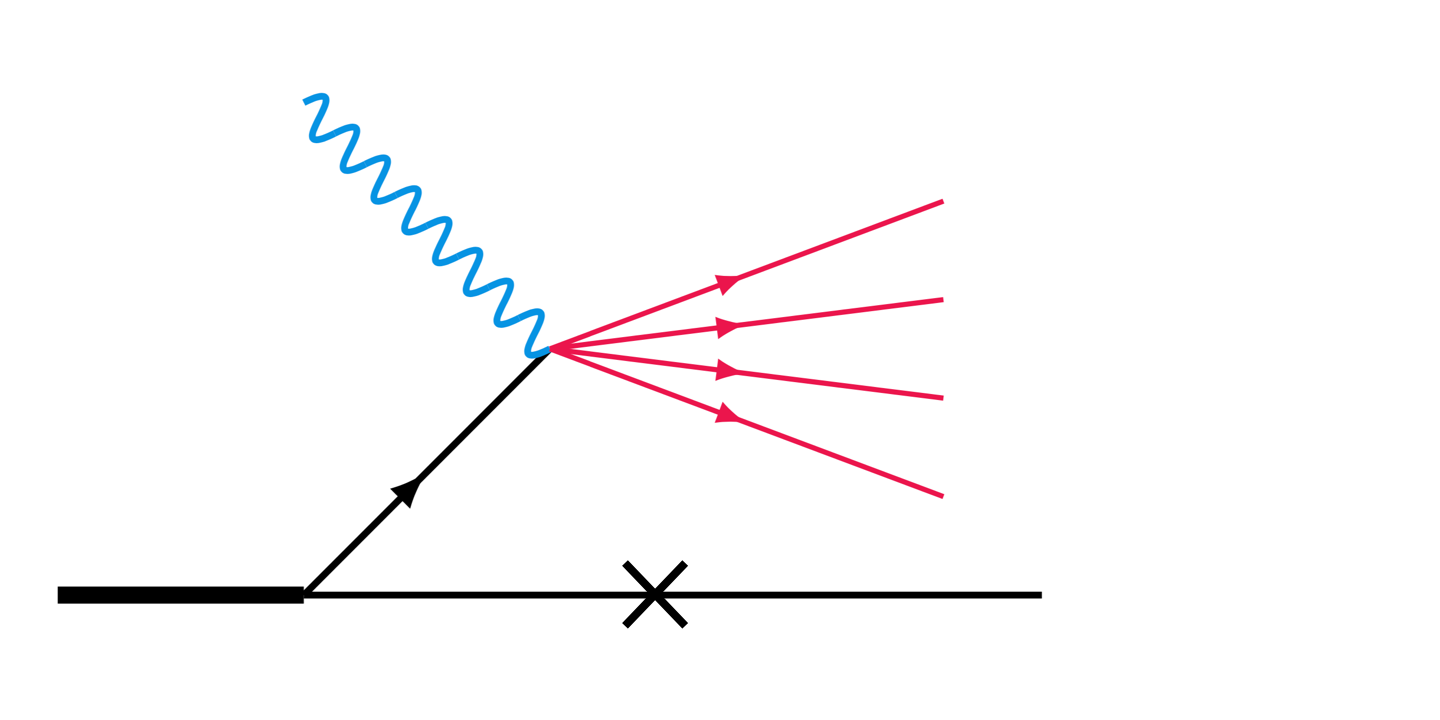
\includegraphics[width=\linewidth]{figures/spec_tag1.png}
		\caption{}
		\label{fig:spec_tag1}
	\end{subfigure}
	\begin{subfigure}[b]{0.4\linewidth}
		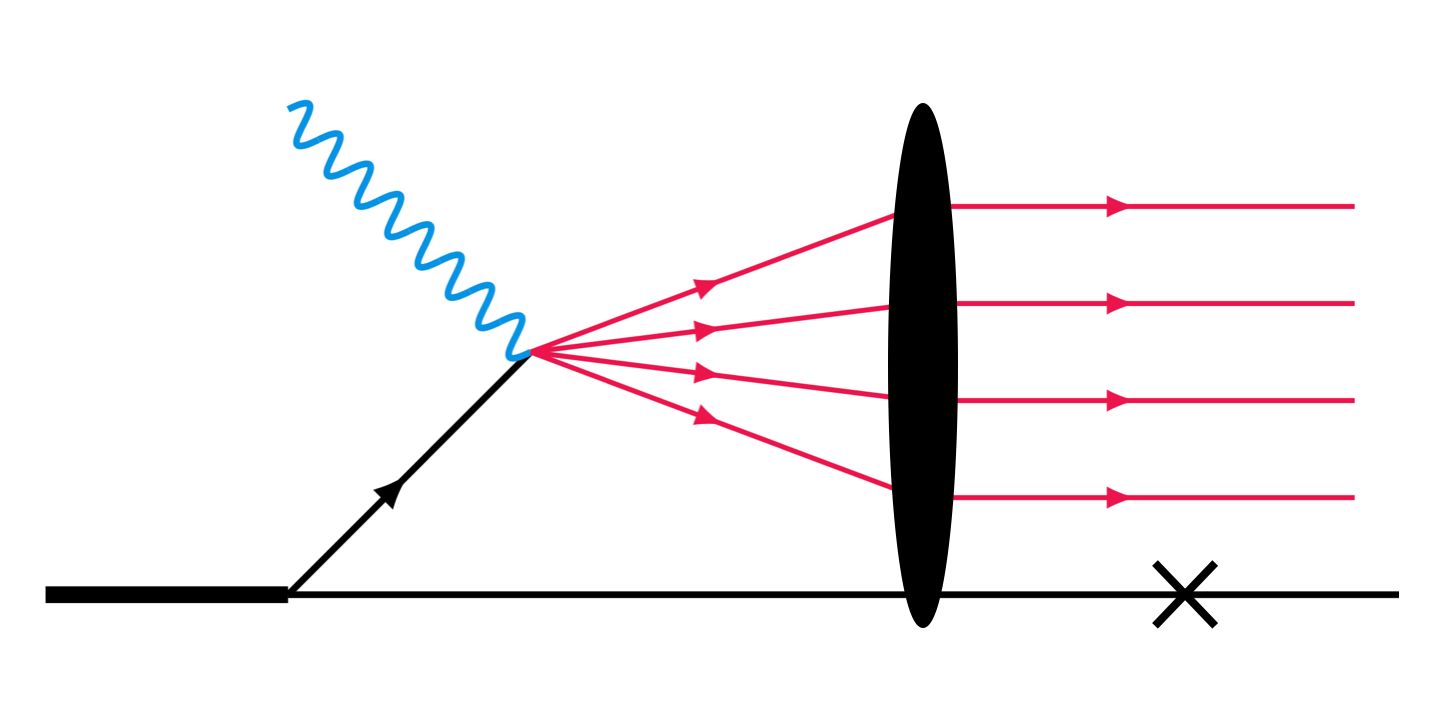
\includegraphics[width=\linewidth]{figures/spec_tag2.png}
		\caption{}
		\label{fig:spec_tag2}
	\end{subfigure}
	\caption{Impulse approximation (a) and final state interaction diagrams (b).}
	\label{fig:spec_tag}
\end{figure}

The assumption in Eq. \ref{eqn:eD_epX} is that the reaction occurs when the momentum of the spectator proton is less than $700$ MeV/c \cite{spec_tag}, where the virtual photon interacts with only one of the bound nucleons. Particles produced from the reaction can interact in the final state with the spectator nucleon. Two diagrams contribute to the cross section: the impulse approximation when the particle debris from the struck nucleon does not interact with the other nucleon (Fig. \ref{fig:spec_tag1}), and the case where rescattering occurs of the recoil nucleon with the other products of the deep inelastic scattering (DIS) interaction (Fig. \ref{fig:spec_tag2}), called final-state interactions.

\subsection{Impulse Approximation}
The ideal interaction for studying the structure of the neutron from DIS from deuterium is the impulse approximation (IA). In the IA, the recoil nucleon is a spectator of the virtual photon $\gamma^*$ scattering off the bound nucleon $N$. Using the Feynman rules, the IA amplitude is
\begin{equation}
\label{eqn:ia_amp}
A_{IA}^{\mu} = \bra{X}J_{em}^{\mu}(Q^2, \nu, p_s) \frac{\slashed{p}_D - \slashed{p}_s + m}{M_N^2 - t}\bar{u}(p_s) \Gamma_D,
\end{equation}
where $J_{em}^{\mu}(Q^2, \nu, p_s)$ represents the electromagnetic DIS operator of the electron scattering off the bound nucleon, $t = (p_D - p_s)^2$, and $\Gamma_D$ is the covariant $D \rightarrow pn$ transition vertex.

If we take the recoil nucleon in Fig. \ref{fig:spec_tag1} on the mass shell and using \cite{spec_tag}
\begin{equation}
\slashed{p}_D - \slashed{p}_s + m \approx \sum_{\mathrm{spins}} u(p_D-p_s)\bar{u}(p_D-p_s),
\end{equation}
we can factorize Eq. \ref{eqn:ia_amp} into two parts: (1) the DIS current of the bound nucleon ($i.e.$ $J_{X,N}^{\mu} = \bra{X} J_{em}^{\mu}(Q^2, \nu, p_s) u(p_D-p_s) $), and (2) the wave function of the deuteron. This factorization provides us with nuclear DIS structure functions through convolution of bound nucleon structure functions ($F_{1D}^{\mathrm{eff}}$ and $F_{2D}^{\mathrm{eff}}$) and the nuclear spectral function $S$, which (following \cite{spec_tag}) are 
\begin{flalign}
\label{eqn:sf_ia}
\nonumber
F_{2D}^{SI}(x, Q^2, \alpha_s, p_s^{\perp}) =& \frac{S(\alpha_s,p_s^{\perp})}{n}\frac{M_N\nu}{pq} \\
\nonumber
& \times \left[(1+\cos \delta)^2\left( \alpha + \frac{pq}{Q^2}\alpha_q \right)^2 + \frac{1}{2}\frac{(p_s^{\perp})^2}{M_N^2} \sin^2\delta \right] F_{2D}^{\mathrm{eff}}(\tilde{x}, Q^2, \alpha_s, p_s^{\perp}), \\
F_{1D}^{SI}(x, Q^2, \alpha_s, p_s^{\perp}) =& \frac{S(\alpha_s,p_s^{\perp})}{n} \left[ F_{1D}^{\mathrm{eff}}(\tilde{x}, Q^2, \alpha_s, p_s^{\perp}) + \frac{(p_s^{\perp})^2}{2pq} F_{2D}^{\mathrm{eff}}(\tilde{x}, Q^2, \alpha_s, p_s^{\perp}) \right],
\end{flalign}
where $\sin^2 \delta = Q^2/\mathbf{q}^2$. In the virtual-nucleon (VN) approximation $n = M_D/2(M_D - E_s)$ and in the light-cone (LC) approximation $n = 2 - \alpha_s$. The modified Bjorken-$x$ is given in the lab frame by
\begin{equation}
\tilde{x} \approx \frac{Q^2}{2M\nu(2 - \alpha)}.
\end{equation}
The nuclear spectral function $S$ gives us the probability of finding an interacting nucleon with momentum ($\alpha$, $p^{\perp}$) in the target and a recoil nucleon with momentum ($\alpha_s$, $p_s^{\perp}$) in the final state of the reaction. In the IA, $\alpha + \alpha_s = 2$ and $\mathbf{p}^{\perp} = -\mathbf{p}_s^{\perp}$. Putting this all together, we can use Eq. \ref{eqn:sf_ia} in \ref{eqn:spec_xsec} to get

\begin{flalign}
\nonumber
\frac{d\sigma}{dxdQ^2d^3p_s/E_s} =& \frac{4\pi \alpha_{em}^2}{xQ^4} \left( 1 - y - \frac{x^2y^2M_N^2}{Q^2} \right) \frac{S(\alpha_s,p_s^{\perp})}{n}\\
\nonumber
&\times  \left( \frac{M_N\nu}{pq} \left[ (1+\cos \delta)^2\left( \alpha + \frac{pq}{Q^2}\alpha_q \right)^2 + \frac{1}{2}\frac{(p_s^{\perp})^2}{M_N^2} \sin^2\delta \right] \right. \\
\nonumber
& \left. \times F_{2D}^{\mathrm{eff}}(\tilde{x}, Q^2, \alpha_s, p_s^{\perp}) +2\tan^2 \left( \frac{\theta}{2} \right) \frac{\nu}{M_N}  \right. \\
& \left. \times \left[ F_{1D}^{\mathrm{eff}}(\tilde{x}, Q^2, \alpha_s, p_s^{\perp}) + \frac{(p_s^{\perp})^2}{2pq} F_{2D}^{\mathrm{eff}}(\tilde{x}, Q^2, \alpha_s, p_s^{\perp}) \right] \right),
\end{flalign}
where $\alpha_q = (\nu - |\mathbf{q}|)/M_N$.

\subsection{Minimizing Final State Interactions}
The IA is an ideal case, particularly for the BONuS12 Experiment, where we desire no interaction between the spectator proton and the hadronic debris created from the $\gamma^*$-neutron interaction within the deuteron. We want to minimize any possibility of final state interactions to ensure that the proton we measure has not participated in the reaction. 

For any process where final state interactions (FSI) may occur, like the BONuS12 Experiment, it is important to understand and describe quantities relevant to the process. The central quantity describing FSI processes is the distorted momentum distribution \cite{FSI}
\begin{equation}
n_{D}^{FSI}(\mathbf{p}_s,\mathbf{q}) = \frac{1}{3} \frac{1}{(2\pi)^3} \sum_{\mathcal{M}_D} \left| \int d\mathbf{r} \Psi_{1,\mathcal{M}_D}(\mathbf{r}) S(\mathbf{r}, \mathbf{q}) \chi_f^+ \exp(-i\mathbf{P}_s \mathbf{r})\right|^2,
\end{equation} 
where $\xi_f$ is the spin function of the spectator nucleon and $S(\mathbf{r},\mathbf{q})$ is the $S$-matrix describing the FSI between the hadronic debris and the spectator. This $S$-matrix is
\begin{equation}
S(\mathbf{r},\mathbf{q}) = 1-\theta(z)\frac{\sigma_{\mathrm{eff}}(z,Q^2,x)(1-i\alpha)}{4\pi b_0^2}\exp \left( -\frac{b^2}{2b_0^2} \right),
\end{equation}
where $\sigma_{\mathrm{eff}}$ is the time-dependent cross section and $\alpha$ is the ratio of real to imaginary part of the forward amplitude. When FSI do not occur $\sigma_{\mathrm{eff}} = 0$, and the usual deuteron momentum distribution is recovered
\begin{equation}
n_{D}(|\mathbf{p}_s|) = \frac{1}{3} \frac{1}{(2\pi)^3} \sum_{\mathcal{M}_D} \left| \int d\mathbf{r} \Psi_{1,\mathcal{M}_D}(\mathbf{r}) \chi_f^+ \exp(-i\mathbf{P}_s \mathbf{r})\right|^2.
\end{equation}

\begin{figure}
	\centering
	\begin{subfigure}[b]{0.4\linewidth}
		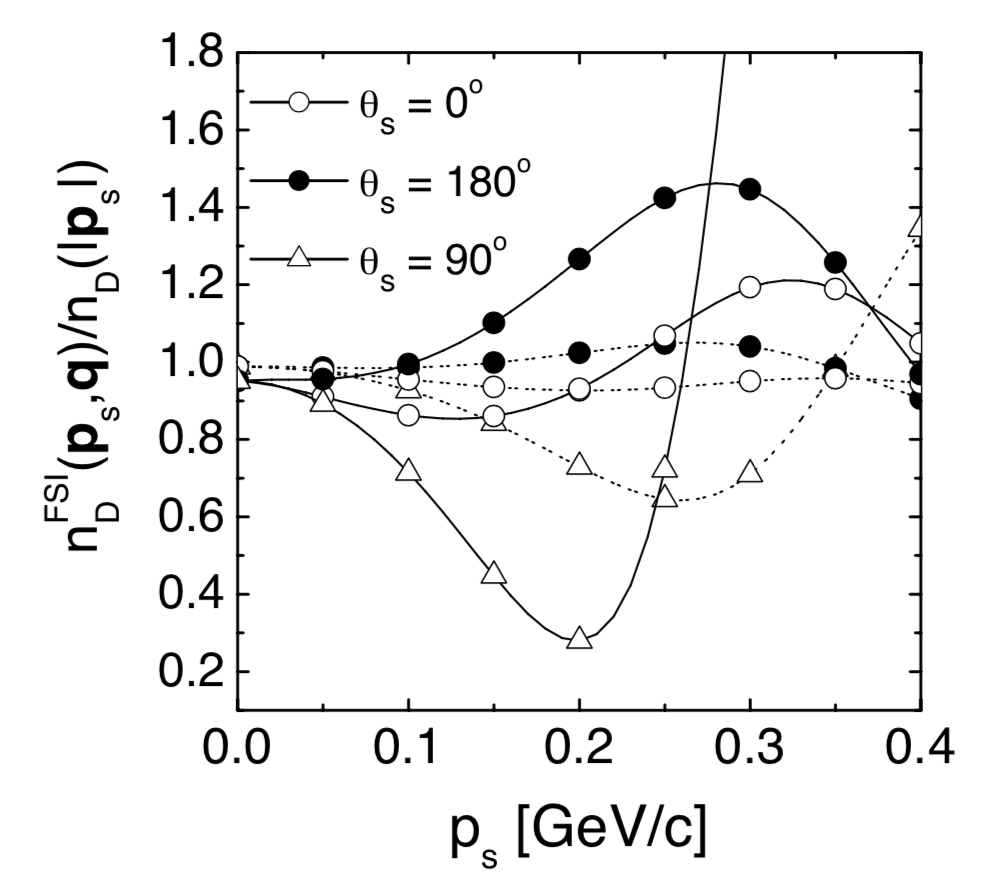
\includegraphics[width=\linewidth]{figures/fsi_p.png}
		\caption{}
		\label{fig:fsi_p}
	\end{subfigure}
	\begin{subfigure}[b]{0.4\linewidth}
		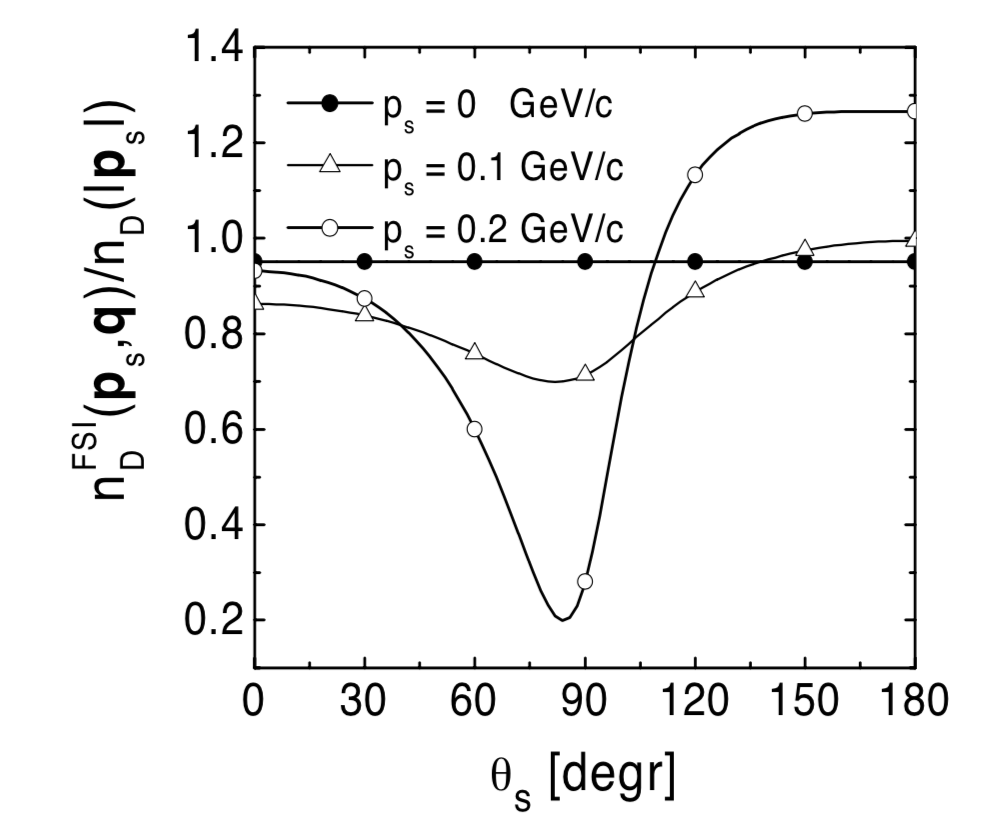
\includegraphics[width=\linewidth]{figures/fsi_th.png}
		\caption{}
		\label{fig:fsi_th}
	\end{subfigure}
	\caption{(a) The Deep Inelastic Scattering ratio $n_{D}^{FSI}/n_D$ with $n_{D}^{FSI}$ and $n_D$, calculated $vs.$ the momentum $p_s \equiv |\mathbf{p}_s|$ of the spectator nucleon emitted at different angles $\theta_s$. The full lines correspond to the $Q^2$- and $z$-dependent debris-nucleon effective cross section $\sigma_{\mathrm{eff}}$, whereas the dashed lines correspond to a constant cross section $\sigma_{\mathrm{eff}} = 20$ mb. (b) The Deep Inelastic Scattering ratio $n_{D}^{FSI}/n_D$ with $n_{D}^{FSI}$ and $n_D$, calculated $vs.$ the emission angle $\theta_s$ of the spectator, for different values of the spectator momentum. Calculations were performed at $Q^2 = 5$ (GeV/c)$^2$ and $x = 0.2$ for the both graphs.}
	\label{fig:fsi}
\end{figure}

To minimize any FSI that may occur in a process like Eq. \ref{eqn:eD_epX}, we look toward the ratio of the distorted $n_{D}^{FSI}$ to deuteron $n_{D}$ momentum distributions. When that ratio goes to unity, final state interactions do not exist. Fig. \ref{fig:fsi_p} shows that ratio as a function of the spectator proton momentum ($p_s$) for various angles ($i.e.$ $\theta_s = 0^{\circ}$, $90^{\circ}$, and $180^{\circ}$). The solid lines correspond to $Q^2$ and $z$-dependent debris-nucleon effective cross section $\sigma_{\mathrm{eff}}$, whereas the dashed lines are for the constant cross section $\sigma_{\mathrm{eff}} = 20$ mb. From this we see that for momenta below 100 MeV/c, all lines begin to converge to unity.

The plot of the $n_{D}^{FSI}/n_{D}$ ratio versus spectator proton scattering angle ($\theta_s$) in Fig. \ref{fig:fsi_th} contains lines for three different values of spectator momenta ($i.e.$ $p_s$ = 0, 100, 200 MeV/c). This plot shows us that for momenta below 100 MeV/c, angles above $100^{\circ}$ minimize FSI. Therefore, in order to minimize FSI in the semi-inclusive ($i.e.$ detecting some, but not all, particles after the interaction) DIS reaction that occurs in the BONuS12 Experiment, spectators protons with momenta below 100 MeV/c at angles above $100^{\circ}$ are detected in coincidence with the scattered electron: $D(e,e',p_s)X$. This allows us to utilize the IA to extract the $F_2^n$ structure function and thus the $F_2^n/F_2^p$ structure function ratio.
